% Anonymised manuscript for the International Journal of Forecasting
% (double-anonymised review).  Author details, funding and declarations are
% in ijf_title.tex; the sections are shared with main.tex.
\documentclass[preprint,review,12pt,authoryear,nonatbib]{elsarticle}
\usepackage{graphicx}
\usepackage{amsmath}
\usepackage{amssymb}
\usepackage[hidelinks]{hyperref}
\usepackage[margin=1in]{geometry}
\usepackage{placeins}
\usepackage{float}
\usepackage[style=authoryear,backend=biber,maxbibnames=6,uniquename=false]{biblatex}
\usepackage{booktabs}
\usepackage{array}
\usepackage{caption}
\usepackage{microtype}
\usepackage{xcolor}
\usepackage{lineno}
\linenumbers

\emergencystretch=1em

% Numbers used in the text (from the experiments).
\newcommand{\nTrain}{184{,}268}
\newcommand{\nTest}{104{,}854}
\newcommand{\nParams}{1{,}805}
% The repository would identify the authors: withheld for review.
\newcommand{\codeurl}{Repository link withheld for anonymous review; the code
and data are provided as supplementary material.}

\addbibresource{ref.bib}

\journal{International Journal of Forecasting}

\begin{document}

\begin{frontmatter}

\title{A Unified Price-and-Demand Model for Cost-Optimal Day-Ahead
Electricity Demand Forecasting: Evidence from the Israeli Market}

\begin{abstract}
Day-ahead electricity is bought before demand is known, and a shortfall is
settled at a price several times higher than a surplus, by a factor that rises
with the price.  The cost-optimal forecast is therefore a quantile of demand
that moves with the price, yet demand and prices are forecast separately and
for accuracy.  We propose a unified model: a small neural network that
forecasts demand and prices from a shared representation and trains the
demand forecast on the price-weighted procurement cost.  On a new open dataset
of the Israeli market, with real day-ahead and synthetic imbalance prices,
the model lowers the excess cost of the test year to \$49.5 million: 6\%
below a joint demand-and-price network trained for accuracy and corrected
afterwards, and 19\% below the operator's corrected forecast.  Replacing the
operator's published forecast would save about \$27 million per year in
Israel, roughly \$1 billion at US scale.
\end{abstract}

\begin{keyword}
Load forecasting \sep Electricity price forecasting \sep
Decision-focused learning \sep Newsvendor problem \sep Imbalance cost \sep
Quantile forecasting \sep Neural networks
\end{keyword}

\end{frontmatter}

\section{Introduction}\label{sec:intro}
The modern electricity grid operates through wholesale markets in which
producers and large consumers interact---directly or through a central
operator---to determine how much power is generated and consumed.  In a
stylised day-ahead market, producers submit offers specifying the quantities of
electricity they are willing to supply at various price points, while suppliers
(and possibly a handful of very large consumers) submit corresponding demand
bids.  A system operator then clears the system by finding the price at which
aggregate supply equals aggregate demand, setting a single clearing price for
each settlement period (typically one hour).  This mechanism promotes economic
efficiency by rewarding low-cost producers and incentivising demand
response~\parencite{stoft2002power, kirschen2018fundamentals}.

Real markets differ considerably in how centralised this process is.  The
Israeli market, which is the setting of this study, is comparatively
centralised: the system operator (Noga) forecasts national demand for each hour
of the following day, and this day-ahead forecast---together with the resulting
price signal---determines how much electricity producers are scheduled to
deliver in each settlement period.  The process is therefore less the
continuously cleared double auction of textbook descriptions and more a
coordinated, forecast-driven dispatch.  Regardless of the precise market design,
however, the day-ahead demand forecast is the pivotal quantity: it is fixed
before real-time demand is known, and its accuracy propagates directly into
generation scheduling and price.

A central challenge in this architecture is that procurement decisions must be
finalised a day in advance, before actual real-time demand is known.  The
accuracy of demand forecasts therefore directly affects the operational
decisions and financial outcomes of all market participants.  It remains an open
question to what extent individual suppliers maintain their own demand models.  A
plausible account of current practice is that, once the operator publishes its
day-ahead demand forecast, each supplier simply draws its own share from that
forecast based on experience, and the market settles on a relatively stable price
that is reasonable on average but may embed sizeable, systematic error margins.
If so, more sophisticated forecasting---whether by the suppliers or by the system
operator---could translate into lower retail prices, which is part of what
motivates the present work.

A system operator that accurately anticipates demand can procure the right
amount of energy at competitive prices.  Inaccurate forecasts, by contrast,
force participants into costly corrective actions in the balancing or real-time
markets, where prices can be dramatically different from day-ahead levels.  It is
worth stressing that these price differences arise from two distinct sources of
uncertainty: errors in predicting \emph{demand}, and errors in predicting
available \emph{production capacity}---the latter being especially pronounced in
systems that rely heavily on variable renewable generation such as solar and
wind~\parencite{morales2014integrating}.  This paper is concerned exclusively
with the first source of differences, uncertainty in day-ahead demand; production-side
uncertainty, while important, is outside our scope.

\subsection{Asymmetric Costs in Electricity Markets}

A critical and often overlooked aspect of electricity demand forecasting is the
\emph{asymmetry} of the costs associated with forecast errors.  When demand is
\emph{overestimated}, the system operator or retailer procures more electricity
than is ultimately needed.  The excess supply can typically be sold back into the
balancing market, curtailed, or stored (if storage is available), resulting in a
relatively modest financial loss.  In deregulated markets with well-functioning
balancing mechanisms, the per-unit cost of over-procurement is generally bounded
and predictable.

When demand is \emph{underestimated}, the cost of error is usually much higher.
The system operator must source additional electricity in the real-time market at
short notice to prevent blackouts.  Real-time prices are typically highly
volatile and can spike to several multiples of the day-ahead price during periods
of scarcity.  In extreme cases, the system may lack sufficient reserve capacity
to meet demand, triggering involuntary load shedding, emergency imports, or the
activation of expensive peaking units.  Beyond the direct financial costs, supply
shortfalls carry significant reliability and regulatory
implications~\parencite{stoft2002power, kirschen2018fundamentals}.

Empirical studies in various electricity markets suggest that the ratio of
under-procurement costs to over-procurement costs, $c_u / c_o$, typically lies in
the range $[5,\,20]$, depending on market structure, regulatory context, and the
availability of real-time resources~\parencite{zhang2022costoriented}.  This
asymmetry fundamentally changes the optimal forecasting problem: rather than
seeking a prediction that minimises expected squared error, a rational market
participant should seek a prediction that minimises expected asymmetric cost.

This decision-theoretic view has developed alongside a substantial body of work
on electricity forecasting more broadly.  \textcite{weron2014electricity}
provides a comprehensive review of the state of the art in electricity price
forecasting, surveying statistical, machine-learning, and hybrid approaches.
While its focus is on price rather than demand, the review highlights the central
role of model selection, loss-function choice, and benchmark comparisons that
also apply in the load-forecasting context.

\textcite{hong2016probabilistic} offer a tutorial review of probabilistic
electric load forecasting, covering methods ranging from regression-based
quantile estimation to ensemble and Bayesian approaches.  Crucially, they argue
that point forecasts are insufficient for operational decision-making and
advocate for full predictive distributions or at least prediction intervals---a
view consistent with the quantile-forecasting objective we adopt.

The practical importance of probabilistic evaluation metrics, and of the pinball
loss in particular, was cemented by the Global Energy Forecasting Competition
2014~\parencite{hong2016gefcom2014}.  GEFCom2014 was the first major forecasting
competition to use pinball loss as its primary scoring rule across the
electricity load, price, wind, and solar tracks.  It established pinball loss as a
community standard and demonstrated that models explicitly optimised for quantile
accuracy substantially outperform those adjusted only post-hoc.

Despite the theoretical clarity of this framing, most practical
forecasting systems in electricity markets continue to use symmetric loss
functions---most commonly mean squared error (MSE) or mean absolute error (MAE)---both for training
predictive models and for evaluating their performance.  This disconnect between
training objective and operational cost constitutes a systematic source of
suboptimality that has received growing attention in the academic
literature~\parencite{wang2019pinball, lin2020asymmetric, wu2021svr,
zhang2022costoriented} but has yet to see widespread adoption in practice.

\subsection{Cost-Oriented and Asymmetric Learning for Load Forecasting}

The theoretical foundation for prediction under asymmetric costs was laid by
\textcite{koenker1978regression}, who introduced \emph{regression quantiles} as a
natural generalisation of sample quantiles to the linear model.  They showed that
minimising the asymmetric pinball loss (equivalently, the ``check function'')
yields an estimator of the conditional $\tau$-quantile of the response, and
established its asymptotic properties.  This result directly underpins our
training objective, which is a pinball loss whose slopes are the
(time-varying) market prices of under- and over-prediction.

\textcite{christoffersen1997optimal} provided the corresponding
decision-theoretic foundation.  They showed that under a general asymmetric loss
function the optimal point forecast is \emph{biased}, and that the optimal amount
of bias is time-varying and depends on higher-order conditional moments such as
conditional variance.  In particular, their analysis implies that any forecast
trained with a symmetric objective (e.g.\ MSE) will be systematically suboptimal
when the true cost structure is asymmetric, even if the conditional mean is
estimated perfectly.

Building on these foundations, a more recent line of work addresses the mismatch
between symmetric training objectives and asymmetric operational costs directly
in the electricity setting, embedding the cost asymmetry into the learning
objective itself rather than correcting for it after the fact.

\textcite{wang2019pinball} trained a Long Short-Term Memory (LSTM) network directly
with the pinball loss to produce probabilistic individual load forecasts.  By
guiding the network to minimise $\mathbb{E}[\mathcal{L}_\tau]$ rather than MSE,
their approach yields calibrated quantile predictions without requiring post-hoc
quantile regression on the residuals.  Their results show improved reliability and
sharpness compared to symmetric-loss baselines.

\textcite{lin2020asymmetric} addressed the related problem of contract-capacity
optimisation for high-voltage consumers, where the electricity pricing structure
is inherently asymmetric: underestimating demand triggers penalty charges at a
higher per-unit rate than overestimating.  They proposed several asymmetric loss
functions derived directly from the Taiwan Power Company's pricing formula, and
demonstrate that LSTM models trained with these loss functions reduce electricity
costs by 0.88\%--2.42\% over symmetric MSE baselines.

\textcite{wu2021svr} extended this idea to support vector regression (SVR),
developing a cost-oriented asymmetric SVR (AsySVR) framework based on a
linear-linear loss function with an insensitivity parameter to improve
generalisation.  Evaluated on New South Wales load data, their asymmetric
framework achieved daily economic cost reductions of 42\%--57\% relative to
standard SVR, underscoring that the choice of loss function can have a large
practical impact on operational outcomes.

\textcite{zhang2022costoriented} further formalised the decision-oriented
perspective on load forecasting, framing the problem explicitly in terms of the
downstream cost incurred by the system operator.  Their cost-oriented framework
bridges the gap between forecast-accuracy metrics and operational objectives, and
provides theoretical justification for replacing standard point-forecast losses
with cost-aware alternatives.

Taken together, this recent body of work establishes that asymmetric, cost-sensitive
training objectives are both theoretically motivated and empirically superior to
symmetric alternatives in electricity applications.  There are, by now, many
works that target asymmetric costs in electricity demand forecasting.  To the
best of our knowledge, however, none of them integrates \emph{both} consumption
and price information into a unified model: the asymmetry is encoded as a
\emph{fixed} cost ratio (a single pinball quantile, or the slopes of one
tariff), and prices play no role either as model inputs or as time-varying
weights in the loss.  In real markets the cost of a forecast error is a
\emph{price}, and the relative cost of under- and over-prediction moves with the
day-ahead price itself, so the cost-minimising quantile changes from one
settlement period to the next (Section~\ref{sec:modeling}).

A related line of \emph{decision-focused} or \emph{value-oriented} learning
trains predictors against the downstream decision cost rather than a
statistical error~\parencite{donti2017taskbased, elmachtoub2022spo}.  In power
systems this idea has mainly been applied to renewable generation, where
forecasts of wind or solar output are trained against day-ahead and
real-time market costs~\parencite{stratigakos2022prescriptive,
zhang2024valueoriented}.  Donti et al.\ also include a grid-scheduling task
driven by load forecasts.  These works establish that market costs can be
optimised end-to-end, but they do not address national demand forecasting with
real market prices, nor do they benchmark against the forecast an experienced
system operator actually deploys.  More practically, cost-aware load forecasting
methods are typically compared with statistical baselines rather than with such
an operational forecast, which leaves open whether cost-aware training improves
upon a strong, real-world forecast.

\subsection{Contributions}

Our work addresses these gaps.  We formulate day-ahead demand forecasting as the
minimisation of the realised procurement cost, where committed energy is paid at
the \emph{real} day-ahead market price and imbalances are settled at
under- and over-prediction prices that depend on it.  We train a single
\emph{price-aware} neural network to minimise this cost end-to-end.  Because
the day-ahead price is set only after suppliers commit, prices are not model
inputs; they enter only through the training loss, from which the model learns
when shortfall tends to be expensive.  We then compare it with symmetric (MSE) models,
fixed-ratio asymmetric models, and post-hoc cost adjustments of both,
including adjustments of the \emph{real} day-ahead forecast published by the
Israeli system operator Noga.  The contributions of this paper are as follows:

\begin{enumerate}
    \item \textbf{A unified price-aware forecasting model.}  To the best of our
          knowledge, this is the first work on national electricity demand
          forecasting that integrates \emph{real} day-ahead market prices into
          the model's training objective, as the time-varying slopes of the
          loss, so that a single model learns the cost-optimal forecast from
          consumption and price data jointly, without requiring prices at
          decision time.

    \item \textbf{A novel open dataset.}  We assemble and release a new dataset
          for the Israeli market that combines 5-minute national demand, the
          operator's real day-ahead demand forecast, real half-hourly day-ahead
          market prices (SMP), and hourly weather from three stations, covering
          April~2023 to December~2025.

    \item \textbf{A price-dependent imbalance-cost model.}  We propose a
          generator of synthetic under- and over-prediction prices that is
          anchored on real day-ahead prices and reproduces the stylised facts
          of electricity imbalance settlement (a cost ratio between 5 and 20
          that increases with the price), and we use it to study the
          sensitivity of our conclusions.

    % TODO: state the outcome once the final experiments are in.
    \item \textbf{Strong baselines, including the operator's forecast.}  We
          compare the unified model with models trained to minimise MSE,
          fixed-ratio asymmetric models, and models that are adjusted to the
          cost after training (a global affine correction and a price-aware
          newsvendor correction), as well as the Noga day-ahead forecast with
          the same adjustments.

    \item \textbf{An estimate of the potential savings in Israel.}  We translate
          the cost reductions into an estimate of the annual saving for the
          Israeli market, in shekels and as a share of the day-ahead energy
          bill, together with its sensitivity to the imbalance-price
          assumptions.

    \item \textbf{An open-source implementation.}  We release our complete code
          and data pipeline, from raw data ingestion through model training and
          evaluation, as open source,\footnote{\url{https://github.com/gkutiel/noga}}
          so that our results can be reproduced and extended.
\end{enumerate}


\section{Related Work}\label{sec:related}
\paragraph*{Cost-oriented load forecasting.}  Quantile
regression~\parencite{koenker1978regression} minimises the asymmetric pinball
loss and estimates a conditional quantile, and under an asymmetric loss the
optimal point forecast is biased~\parencite{christoffersen1997optimal}.  The
pinball loss became a standard in energy forecasting with
GEFCom2014~\parencite{hong2016gefcom2014, hong2016probabilistic}.  Several
works train load forecasters directly on an asymmetric cost: an LSTM trained
on the pinball loss~\parencite{wang2019pinball}, LSTMs trained on losses
derived from an asymmetric tariff, which cut electricity costs by
0.9--2.4\%~\parencite{lin2020asymmetric}, an asymmetric support vector
regression~\parencite{wu2021svr}, and a cost-oriented formulation of load
forecasting~\parencite{zhang2022costoriented}.  In all of them the asymmetry
is \emph{fixed}---one quantile, or the slopes of one tariff---and prices play
no role in the model.

\paragraph*{Joint forecasting of load and price.}  Load and price are
strongly coupled, and several models forecast them together:
\textcite{shayeghi2015simultaneous} with a multi-output least-squares SVM on
the NYISO, NSW and PJM markets, and \textcite{li2024joint} with a multi-task
network that shares layers across source, load and price.  These models are
trained for statistical accuracy: their demand forecast targets the
conditional mean, and the predicted price plays no role in how the forecast
trades shortfall against surplus.  Price forecasting on its own has a large
literature~\parencite{weron2014electricity}, likewise accuracy-oriented.

\paragraph*{Decision-focused learning.}  Decision-focused or value-oriented
learning trains predictors against the cost of a downstream decision rather
than a statistical error~\parencite{donti2017taskbased, elmachtoub2022spo};
the feature-based newsvendor~\parencite{ban2019bignewsvendor} learns an order
quantity directly from features under fixed costs.  In power systems the idea
has been applied to wind and solar forecasts traded in
markets~\parencite{stratigakos2022prescriptive, zhang2024valueoriented} and to
load forecasts for a downstream dispatch~\parencite{donti2017taskbased,
han2020lfednet}.  These works treat the cost parameters as given rather than
predicting them, and none addresses national demand with real market prices
or benchmarks against the forecast an operator actually uses.

\paragraph*{The gap.}  After a search of these three literatures we found no
model that \emph{unifies} them: one that forecasts the prices together with
the demand and trains the demand forecast on the price-weighted cost, so that
the decision follows the model's own price expectations.  We therefore
compare against the strongest representative of each line: a joint
load-and-price network trained for accuracy whose own price forecasts then set
the margin, a fixed-asymmetry (pinball) model, and accuracy-trained models
corrected to the cost after training.


\section{Problem Formulation}\label{sec:modeling}
\subsection{Problem Formulation}

In day-ahead electricity procurement, a market participant must commit to a
quantity $p_t$ for every settlement slot $t$ of the following day before
observing the actual demand $y_t$.  Committed energy is paid at the day-ahead
price; any mismatch is settled after the fact at less favourable prices.  We
model $y_t$ as a random variable whose conditional distribution is
\emph{unknown} and must be learned from data; we make no parametric assumption
about its form.

\paragraph*{Price-based cost.}  Let $\pi^{\mathrm{DA}}_t$ denote the day-ahead
price, $\pi^{u}_t$ the price paid for each unit of shortfall (under-prediction),
and $\pi^{o}_t$ the cost of each unit of surplus (over-prediction), with
\begin{equation}
    \pi^{u}_t \;>\; \pi^{\mathrm{DA}}_t \;>\; \pi^{o}_t \;>\; 0.
    \label{eq:price-order}
\end{equation}
The total realised cost of procuring $p_t$ when demand turns out to be $y_t$ is
\begin{equation}
    C_t(p_t, y_t) =
        \pi^{\mathrm{DA}}_t \min(y_t, p_t)
        + \pi^{u}_t \,(y_t - p_t)^{+}
        + \pi^{o}_t \,(p_t - y_t)^{+},
    \label{eq:cost}
\end{equation}
where $(z)^{+}=\max(0,z)$.  Since the consumed energy $\pi^{\mathrm{DA}}_t y_t$
must be paid regardless of the forecast, it is convenient to work with the
\emph{excess cost} above a perfect forecast,
\begin{equation}
    E_t(p_t, y_t) = C_t(p_t,y_t) - \pi^{\mathrm{DA}}_t y_t
    = \underbrace{(\pi^{u}_t - \pi^{\mathrm{DA}}_t)}_{c^{u}_t}\,(y_t - p_t)^{+}
    + \underbrace{\pi^{o}_t}_{c^{o}_t}\,(p_t - y_t)^{+}.
    \label{eq:excess}
\end{equation}
Equation~\eqref{eq:excess} is a pinball loss whose two slopes, $c^u_t$ and
$c^o_t$, are \emph{prices} that vary from slot to slot.

\paragraph*{Information structure.}  We assume that the day-ahead price is the
market-clearing price (the Israeli system marginal price, SMP) and that it is
known when $p_t$ is chosen, as is the over-prediction price $\pi^o_t$.  The
under-prediction price $\pi^u_t$, in contrast, is revealed only in real time
and is \emph{not} available to the forecaster.

\paragraph*{Goal.}  The objective is to choose $p_t$ that minimises the
\emph{expected total cost} $\mathbb{E}[C_t \mid \mathcal{I}_t]$ given the
information $\mathcal{I}_t$ available at decision time---not the expected
prediction error.

\subsection{Optimal Decision: a Price-Dependent Quantile}%
\label{sec:newsvendor}

For fixed prices, Equation~\eqref{eq:excess} is the classical
\emph{newsvendor} problem~\parencite{arrow1951optimal}.  Since $E_t$ is linear
in $\pi^u_t$, the unknown under-prediction price enters the expected cost only
through its conditional mean $\bar\pi^u_t = \mathbb{E}[\pi^u_t \mid
\mathcal{I}_t]$, and the expected cost is minimised by the critical fractile
\begin{equation}
    p^*_t = F_t^{-1}(\tau_t), \qquad
    \tau_t = \frac{\bar c^{u}_t}{\bar c^{u}_t + c^{o}_t}
           = \frac{\bar\pi^{u}_t - \pi^{\mathrm{DA}}_t}
                  {\bar\pi^{u}_t - \pi^{\mathrm{DA}}_t + \pi^{o}_t},
    \label{eq:optimal_threshold}
\end{equation}
where $F_t$ is the conditional distribution of demand.  Two consequences
motivate this paper:
\begin{enumerate}
    \item \textbf{The target quantile moves with the price.}  When imbalance
          prices are a function of the day-ahead price, so is $\tau_t$.  A
          model trained with a symmetric loss (targeting the mean or median)
          or with a fixed-ratio pinball loss (targeting a constant quantile)
          cannot track $\tau_t$.
    \item \textbf{Errors in expensive slots matter more.}  The slopes of
          Equation~\eqref{eq:excess} scale with the price level, so a
          kilowatt-hour of error during a price spike costs many times more
          than one at night.  A cost-trained model allocates its capacity
          accordingly; an MSE-trained model weighs all slots equally.
\end{enumerate}
A \emph{unified} model that receives the known prices as input and is trained
on Equation~\eqref{eq:excess} with the realised prices addresses both points at
once: by the linearity argument above, training against the realised $\pi^u_t$
yields, in expectation, the same minimiser as training against its unknown
conditional mean.

\subsection{Synthetic Imbalance Prices}
\label{sec:synthetic-prices}

The day-ahead prices in our study are the \emph{real} Israeli SMP values
(Section~\ref{sec:dataset}).  Real imbalance prices, however, are not
published for the Israeli market, so we generate synthetic over- and
under-prediction prices that satisfy Equation~\eqref{eq:price-order} and the
following stylised facts:
\begin{itemize}
    \item the cost of surplus is roughly a fixed fraction of the day-ahead
          price;
    \item the price of shortfall is a non-linear, convex and noisy function of
          the day-ahead price---scarcity is expensive exactly when the system
          is already tight;
    \item the under/over price ratio $\pi^u_t/\pi^o_t$ lies in $[5, 20]$ and is
          roughly increasing in the day-ahead price, in line with the cost
          asymmetries reported for electricity
          procurement~\parencite{zhang2022costoriented, weron2014electricity}.
\end{itemize}
Concretely, for each 30-minute settlement period we draw
\begin{align}
    \pi^{o}_t &= \alpha\,(1+\varepsilon_t)\,\pi^{\mathrm{DA}}_t,
        & \varepsilon_t &\sim \mathcal{N}(0, \sigma_o^2), \\
    r_t &= \operatorname{clip}\!\Big(
        \big(r_{\min} + (r_{\max}-r_{\min})\,u_t^{\gamma}\big)\,e^{\eta_t},\;
        r_{\min},\, r_{\max}\Big),
        & \eta_t &\sim \mathcal{N}(0, \sigma_u^2), \\
    \pi^{u}_t &= r_t\,\pi^{o}_t,
\end{align}
where $u_t\in[0,1]$ is the position of $\log\pi^{\mathrm{DA}}_t$ between its
5th and 99th percentiles.  We use $\alpha=0.3$, $\gamma=2$, $\sigma_o=0.03$,
$\sigma_u=0.15$, $r_{\min}=5$ and $r_{\max}=20$.  Because $\alpha r_{\min}>1$,
the ordering~\eqref{eq:price-order} holds in every slot, and $\pi^u_t =
\alpha(1+\varepsilon_t)\,r_t\,\pi^{\mathrm{DA}}_t$ is the day-ahead price times
an increasing convex multiplier.  The over-prediction price is treated as known
to the model; the noise $\eta_t$ makes the under-prediction price unknown at
decision time.  Figure~\ref{fig:tau-vs-price} shows the resulting
cost-optimal quantile: it ranges from about $0.6$ in cheap night-time slots to
about $0.94$ during price spikes.  Section~\ref{sec:sensitivity} varies all
generator parameters.

\begin{figure}[H]
    \centering
    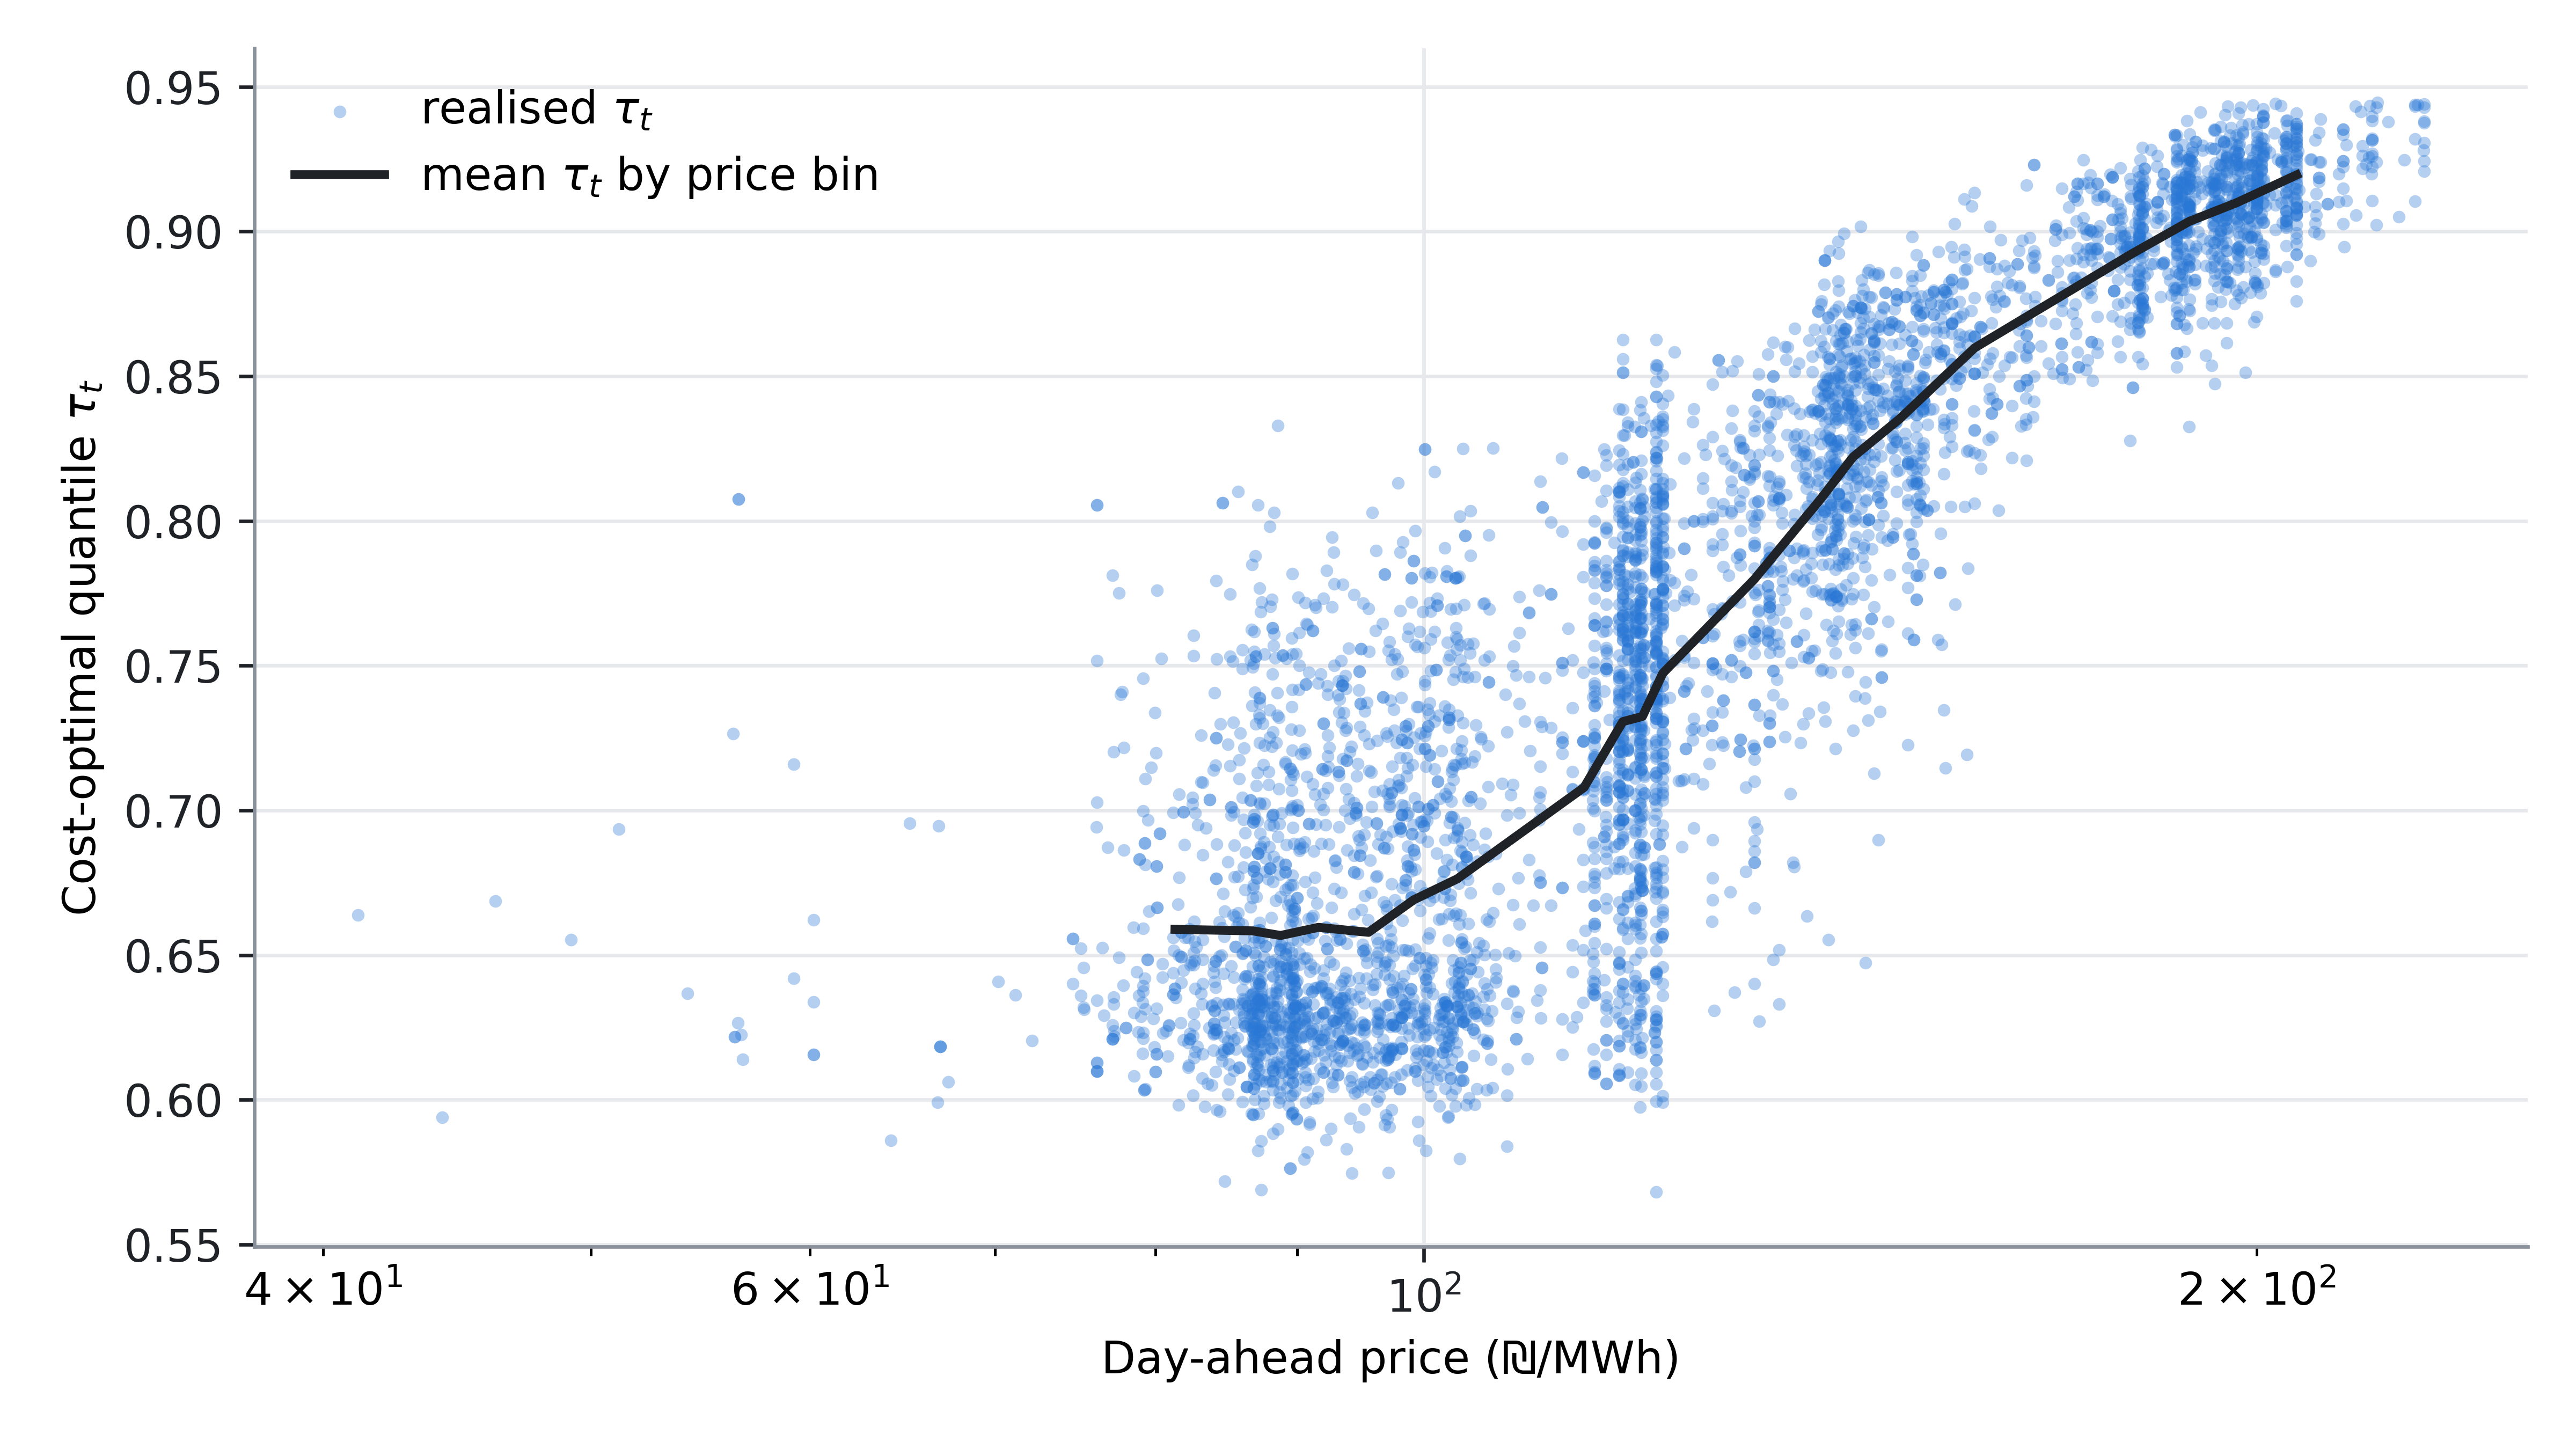
\includegraphics[width=0.8\linewidth]{plot/tau_vs_price.png}
    \caption{Cost-optimal quantile $\tau_t$
             (Equation~\eqref{eq:optimal_threshold}) against the real
             day-ahead price on the test year.  Points are realised values
             (including the unknown noise in $\pi^u_t$); the line is the
             estimate $\hat\tau$ available at decision time.}
    \label{fig:tau-vs-price}
\end{figure}


\section{The Unified Model}\label{sec:architecture}
The objective of this study was to determine whether a single demand forecaster
trained end-to-end on the realised procurement cost, with prices used only in
the training loss (Section~\ref{sec:modeling}) can outperform models
trained to minimise MSE, models trained with a fixed cost asymmetry, post-hoc
cost adjustments of both, and the real operational forecast of the Israeli
system operator.  This section describes the dataset
(Section~\ref{sec:dataset}), the neural architecture and the training
objectives we compare, the post-hoc cost adjustments, and the protocol
under which they are evaluated (Section~\ref{sec:model-training}).

\subsection{Dataset}
\label{sec:dataset}
\subsection{The Israeli Electricity Market}
\label{sec:israel}

Israel is a small country (about 20{,}770~km\textsuperscript{2}, 10.2~million
people) whose population is highly concentrated: most of it lives on the
narrow Mediterranean coastal plain, a strip of about 150~km from Haifa through
the Tel~Aviv metropolitan area to Ashdod, with Jerusalem the main inland
centre (Figure~\ref{fig:pop-density}).  The weather at Haifa, Tel~Aviv and
Jerusalem therefore describes the conditions under which most of the
electricity is consumed.  The climate is hot in summer and mild in winter,
and 96.5\% of households have air conditioning, so demand is driven by
cooling and, to a lesser extent, heating: it peaks in July--August, with a
secondary peak in January--February.  The working week runs from Sunday to
Thursday; Friday and Saturday are the weekend.

The grid is an \emph{electricity island}, with no significant interconnection
to neighbouring countries, so every shortfall must be covered by domestic
reserves.  The market is centralised.  The independent system operator, Noga,
forecasts the national demand for every period of the next day; this
day-ahead forecast, together with the resulting system marginal price (SMP),
determines how much each producer is scheduled to generate.  The day-ahead
demand forecast is thus the pivotal quantity: it is fixed before the demand is
known, and its errors are corrected in real time at a premium.  With about
80~TWh per year and an average load of 9.2~GW, the market is small: a few
percent of the US market.

\begin{figure}[t]
    \centering
    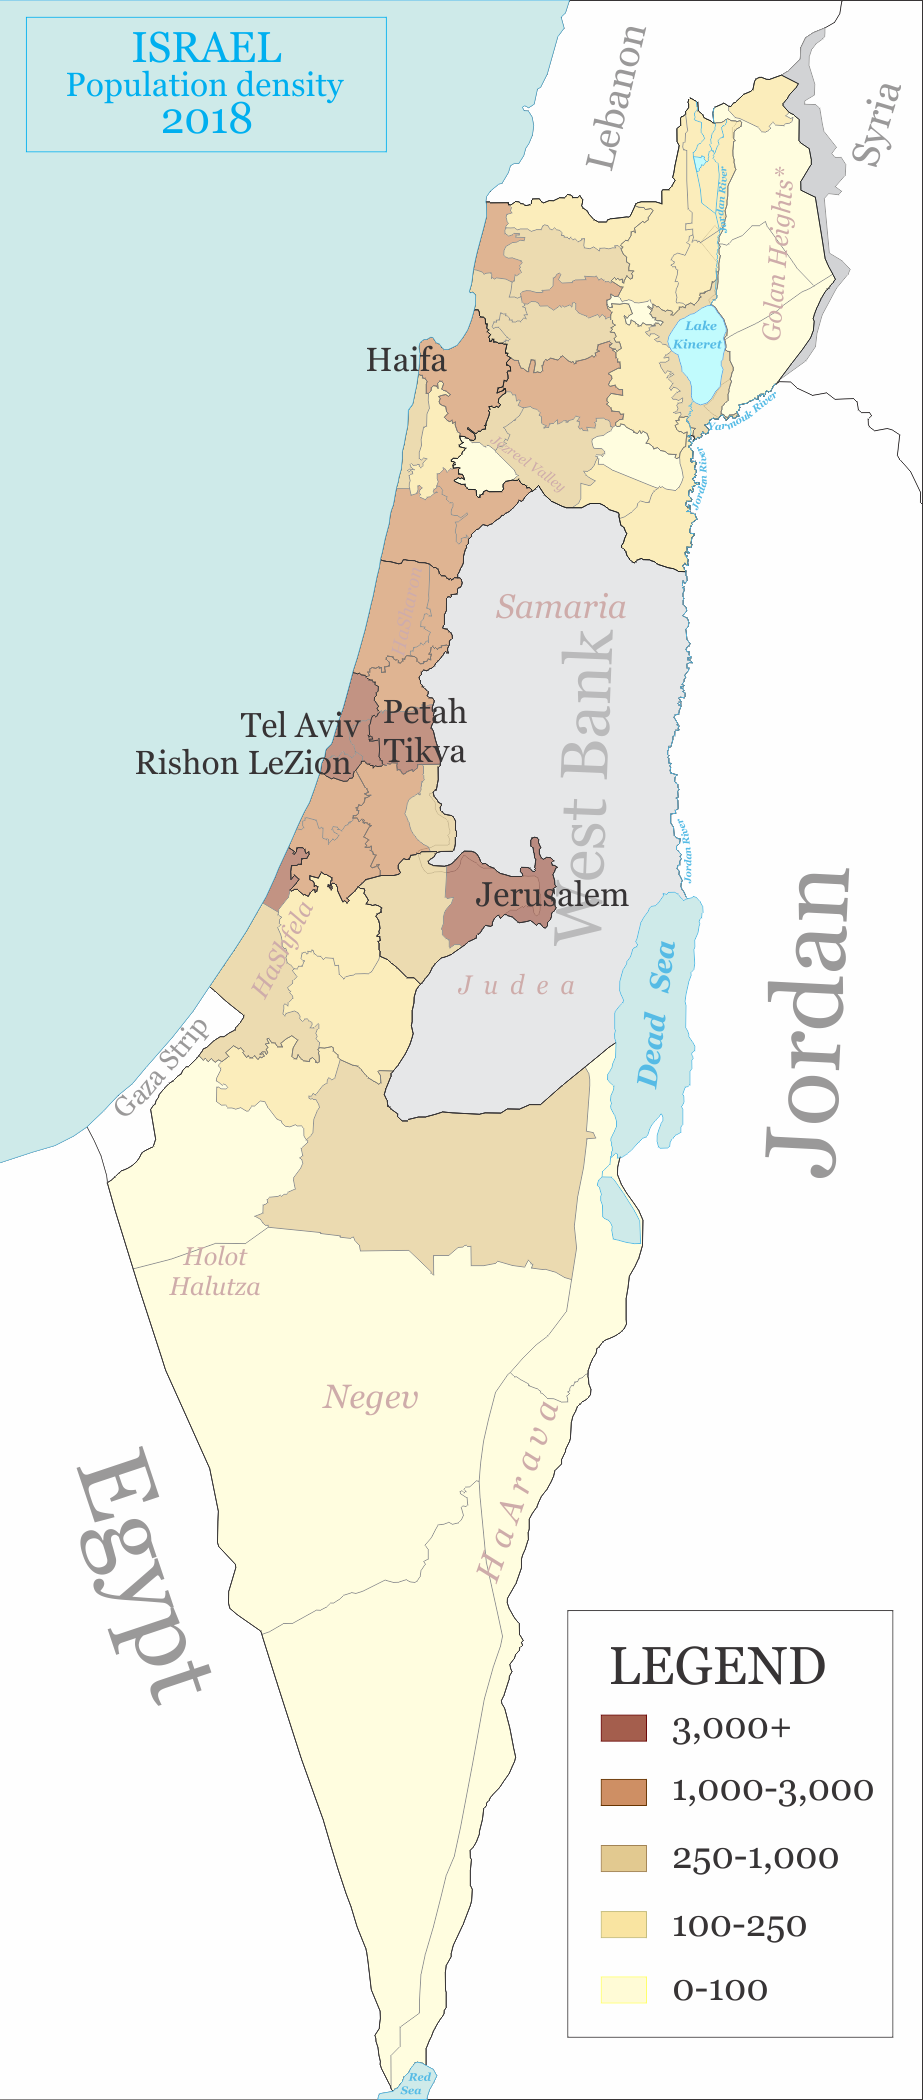
\includegraphics[height=0.42\textheight]{plot/Israel_population_density_2018.png}
    \caption{Population density of Israel (2018, people per km\textsuperscript{2}).
             The coastal plain from Haifa to Ashdod holds most of the
             population; we use the weather at Haifa, Tel~Aviv and
             Jerusalem.}
    \label{fig:pop-density}
\end{figure}

\subsection{The Dataset}

We combine three sources at a common 5-minute resolution, from 1~April~2023
to 31~December~2025; to our knowledge this is the first public dataset of the
Israeli market that aligns them.

\begin{itemize}
    \item \textbf{Demand and the operator's forecast} (Noga, the Israeli
          system operator~\parencite{noga}): national demand every 5~minutes
          and the \emph{real} day-ahead forecast Noga publishes and uses in
          the market---a strong, operational baseline.
    \item \textbf{Day-ahead prices} (Noga~\parencite{noga_smp}): the
          half-hourly unconstrained system marginal price (SMP), the
          market-clearing price $\pi^{\mathrm{DA}}_t$; each 5-minute slot gets
          the price of its settlement period.  (The constrained SMP adds
          redispatch spikes caused by local transmission limits, which a
          national forecast does not affect.)  It averages
          137.5~\textsc{nis}/MWh (\$39.9/MWh) and ranges from 41 to 505.
    \item \textbf{Weather} (Israel Meteorological Service~\parencite{ims}):
          temperature, wet-bulb temperature and relative humidity at Haifa,
          Jerusalem and Tel~Aviv (Figure~\ref{fig:pop-density}).
\end{itemize}

Table~\ref{tab:dataset-stats} summarises the data.  The average load is
9{,}167~MW (about 80~TWh per year).

\paragraph*{The operator's forecast is built for accuracy.}  Noga's forecast
is accurate ($R^2\approx0.98$) and, like a model trained on the squared error,
unbiased and nearly symmetric (Figure~\ref{fig:noga-errors}): the mean error
is $+25$~MW against a standard deviation of 436~MW, and demand exceeds the
forecast in 53\% of the slots.  For accuracy this is ideal; for cost it is
not.  With shortfalls several times more expensive than surpluses, the
cost-optimal forecast is a high quantile (Section~\ref{sec:newsvendor}), and a
forecast centred on the mean falls short about half of the time.

\paragraph*{The uncertainty is not uniform.}  The cost-optimal margin
$F_t^{-1}(\tau_t)-\mathbb{E}[y_t]$ grows with the spread of the demand as
well as with the price.  This spread varies widely: the operator's error
ranges from 1.8\% to 4.8\% MAPE across the hours of the week (standard
deviation 181 to 658~MW, Figure~\ref{fig:error-heatmap}).  It is highest on
the weekend mornings, Friday and Saturday 8:00--15:00, and lowest at night.
A single margin cannot fit both, and a correction per hour of the day (C2,
Section~\ref{sec:compared}) cannot tell a Friday from a Tuesday.  A model
that sees the calendar, the weather and yesterday's price can set its margin
from both the uncertainty and the price.

\begin{figure}[t]
    \centering
    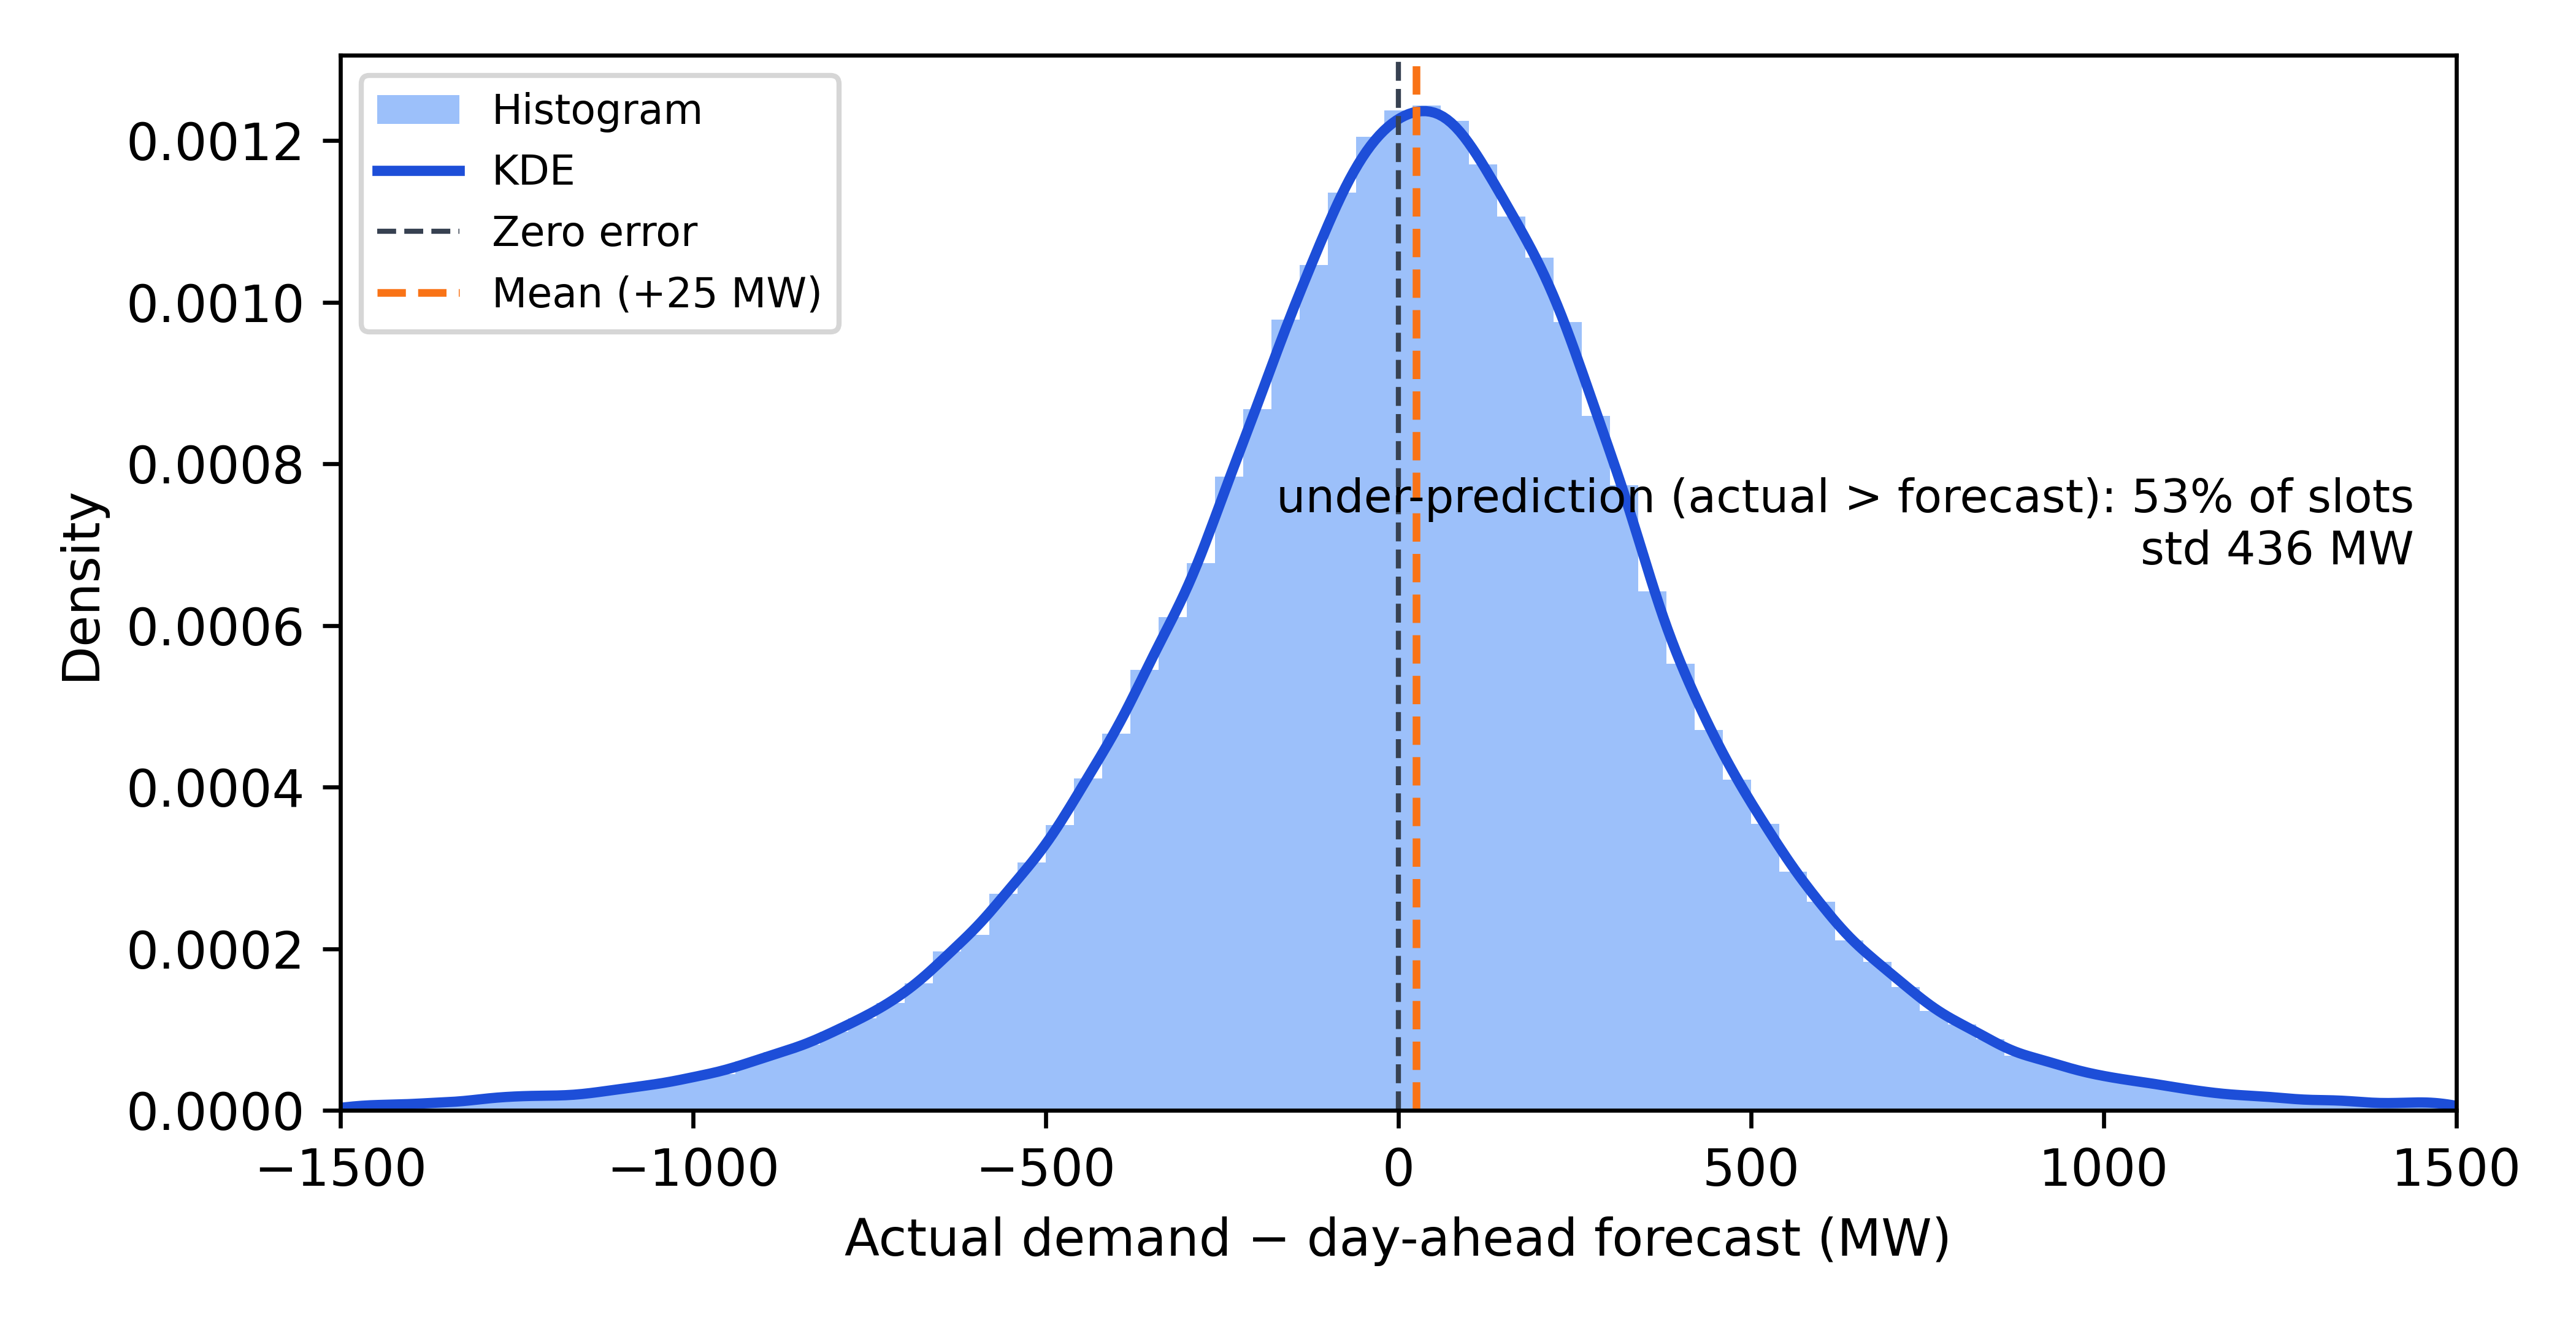
\includegraphics[width=0.85\linewidth]{plot/demand_vs_forecast_kde_histogram.png}
    \caption{Error of the operator's day-ahead forecast (actual minus
             forecast, 5-minute slots, April 2023--December 2025, shown
             within $\pm$1{,}500~MW).  Like a forecast trained on the squared
             error, it is centred near zero and falls short in about half of
             the slots, far from the high quantile that the asymmetric cost
             calls for.}
    \label{fig:noga-errors}
\end{figure}

\begin{figure}[t]
    \centering
    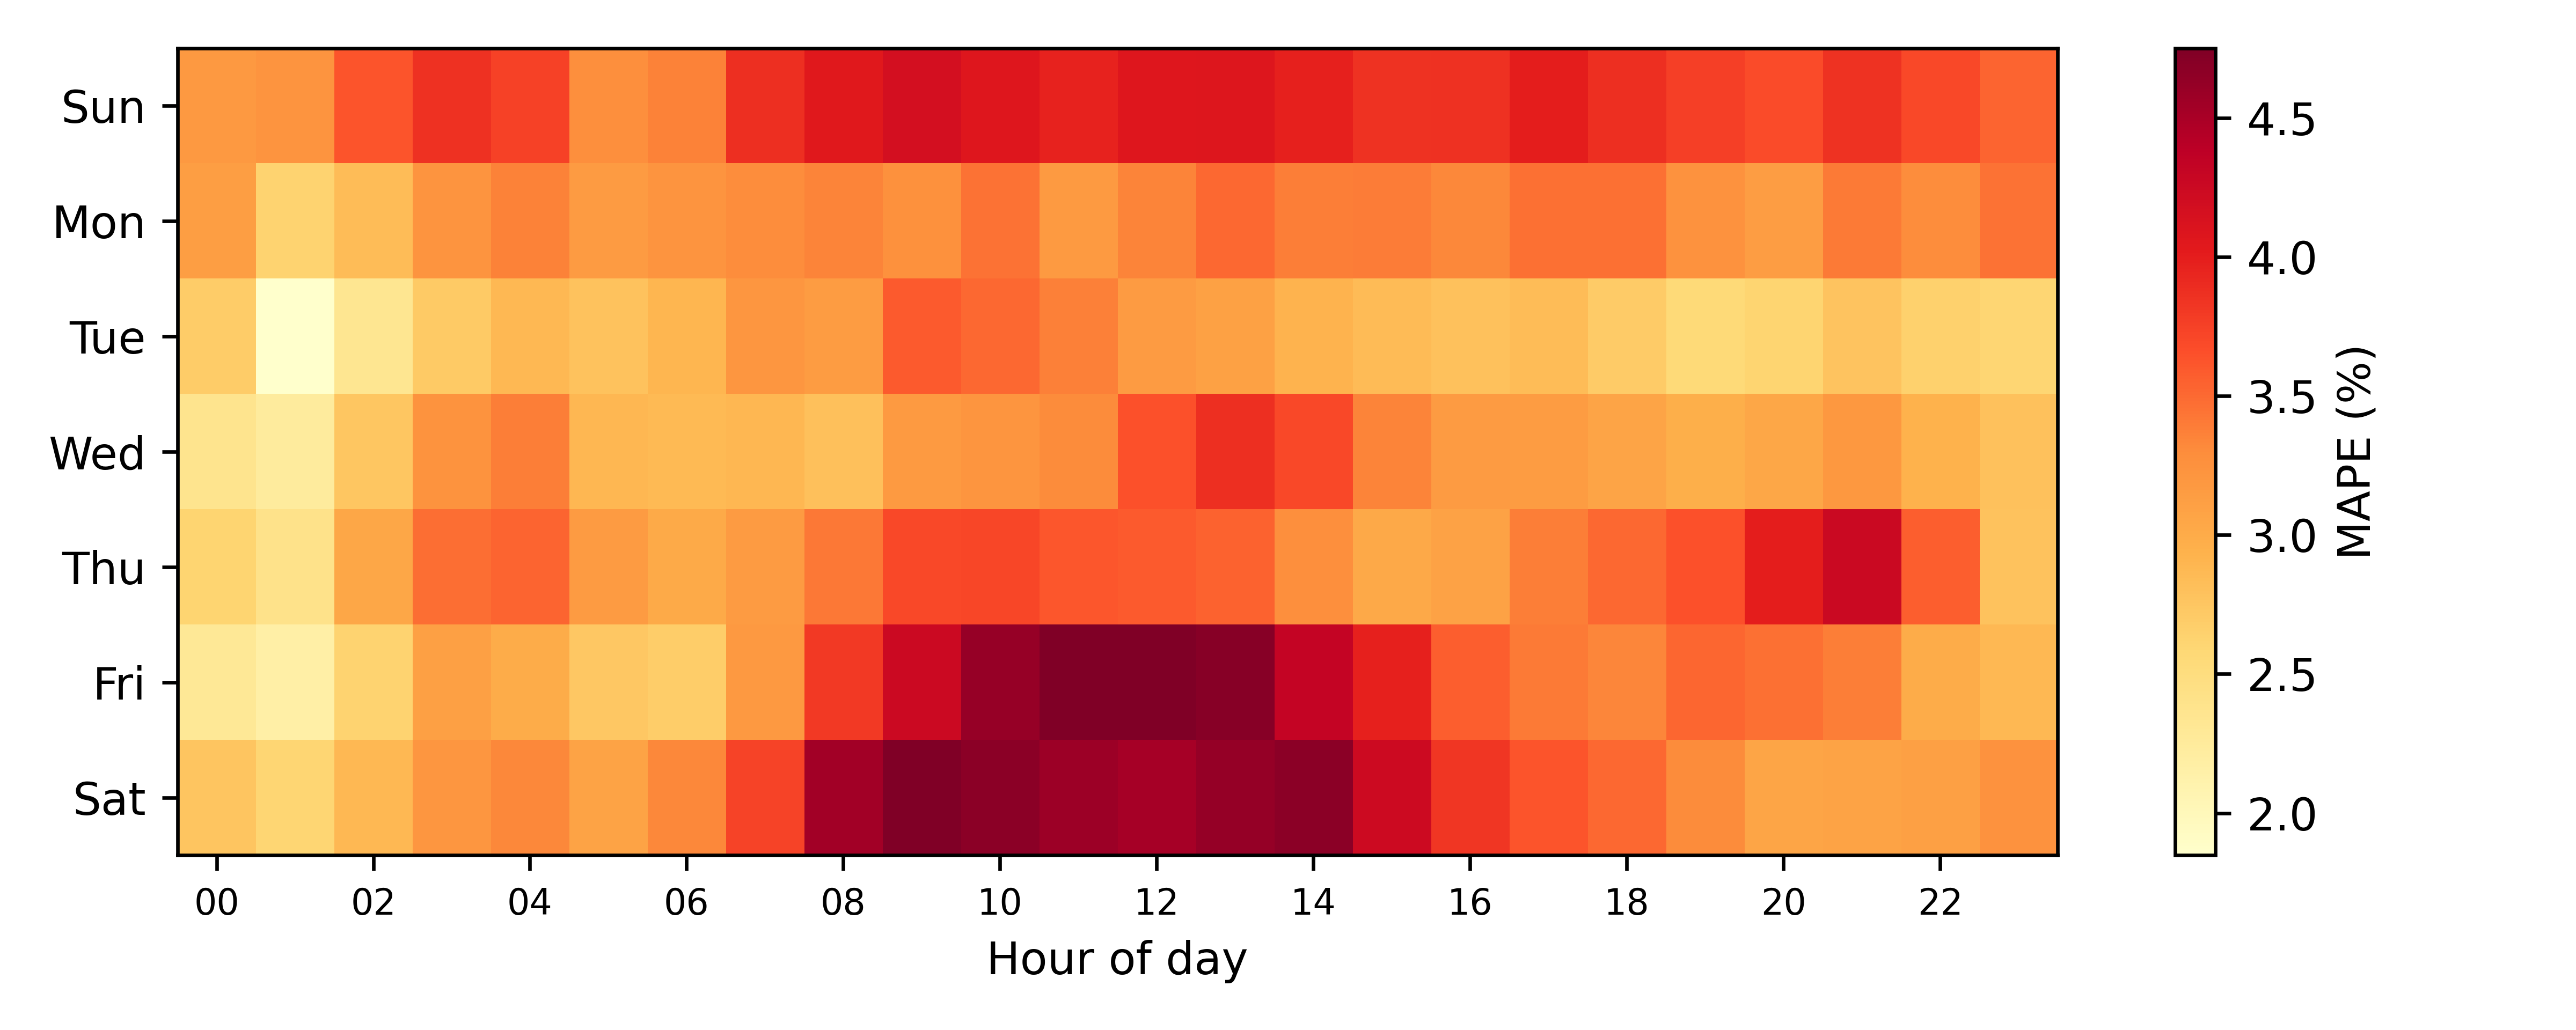
\includegraphics[width=0.9\linewidth]{plot/error_heatmap_percent.png}
    \caption{Mean absolute percentage error of the operator's day-ahead
             forecast by day of week and hour of day.  The uncertainty, and
             with it the cost-optimal margin, varies with the calendar: it is
             highest on the weekend (Friday--Saturday) mornings.}
    \label{fig:error-heatmap}
\end{figure}

\begin{table}[t]
    \centering
    \small
    \caption{Daily summary statistics (1{,}006 days).  $^{*}$Three days with
    an anomalous published forecast (17--19 June 2024) are excluded.}
    \label{tab:dataset-stats}
    \begin{tabular}{lrrrrr}
        \toprule
        \textbf{Variable} & \textbf{Mean} & \textbf{Std} &
        \textbf{Min} & \textbf{Median} & \textbf{Max} \\
        \midrule
        Demand (GWh/day)                       & 219.9 & 37.4 & 147.8 & 211.8 & 342.4 \\
        Operator forecast error (GWh/day)$^{*}$ & $+0.6$ & 6.3 & $-40.1$ & $+0.6$ & $+31.4$ \\
        Day-ahead price (\textsc{nis}/MWh)     & 138 & 26 & 85 & 133 & 245 \\
        Temperature, Tel~Aviv ($^\circ$C)      & 23.2 & 4.8 & 9.6 & 23.7 & 32.1 \\
        \bottomrule
    \end{tabular}
\end{table}

\subsection{Compared Models}
\label{sec:compared}

The data are split chronologically: training on April~2023--December~2024
(\nTrain{} slots) and testing on 2025 (\nTest{} slots).  All learned models
share the network of Figure~\ref{fig:model}, so differences come from how
demand and prices enter training, not from the architecture:

\begin{itemize}
    \item \textbf{MSE}: demand only, trained on the squared error---the
          conventional accuracy-oriented forecaster.
    \item \textbf{Pinball opt}: demand only, trained on the pinball loss at
          the single best constant quantile,
          $\tau^*=\mathbb{E}[c^u]/(\mathbb{E}[c^u]+\mathbb{E}[c^o])=0.864$
          from the training prices---the fixed-asymmetry approach of the
          cost-oriented literature.
    \item \textbf{Joint MSE}: the full network, with the price head, but with
          the demand trained on the squared error---a joint load-and-price
          forecaster trained for accuracy~\parencite{shayeghi2015simultaneous,
          li2024joint}.
    \item \textbf{Unified cost model} (proposed): the full network trained on
          the excess cost and the price loss.
    \item \textbf{Noga}: the operator's published forecast.
\end{itemize}

\paragraph*{Post-hoc corrections.}  To test whether the benefit can be had
more cheaply, we correct the accuracy-trained forecasts to the cost after
training, fitting each correction on the model's own training-set forecasts
at the realised prices: \textbf{C1}, a global affine map $a\hat y+b$;
\textbf{C2}, an affine map per hour of the day, started from the exact
cost-optimal shift of each hour (a cost-weighted quantile of its errors,
Equation~\eqref{eq:weighted_quantile}); and, for Joint MSE, a
\textbf{$\hat\tau$ shift}, which uses the model's own price forecasts: the
training slots are split into deciles of the predicted quantile
$\hat\tau_t$ (Equation~\eqref{eq:optimal_threshold}), and each decile gets its
own cost-optimal shift.  This last baseline is the textbook
\emph{forecast-then-optimise} use of a joint load-and-price forecast.  The
proposed model is never corrected.

\paragraph*{Evaluation.}  The metric is the excess cost
(Equation~\eqref{eq:excess}) on the test year, split into its under- and
over-prediction parts, in million US dollars per year at
3.45~\textsc{nis}/\$ (the 2025 average).  We also report MAE, RMSE and
coverage $P(y_t\le p_t)$.  Each learned model is trained with three seeds
(mean $\pm$ standard deviation), with one draw of the imbalance prices.
Differences in daily cost (averaged over seeds) are tested with the
Diebold--Mariano test~\parencite{diebold1995comparing} with a Newey--West
variance (lag 7 days).


\subsection{Model Training}
\label{sec:model-training}

All model variants share the same architecture: the prediction is expressed as
a \emph{soft attention} over a short window of recent historical demand values
plus a learned additive correction.  Weather conditions (air temperature, wet-bulb
temperature, and relative humidity --- all raw fields reported directly by the
IMS --- at three meteorological stations),
and temporal patterns (time of day, day of week, month of year) jointly
determine both the attention weights and the correction term.  Temporal
features are encoded via learned embeddings; weather features enter as
continuous inputs.  Prices are never model inputs: the day-ahead price is set
only after the procurement decision, so prices are used only in the training
loss and in the evaluation.  The model
operates at 5-minute granularity and produces a day-ahead forecast.  The
variants differ \emph{only} in their training objective, so that any
difference in cost can be attributed to it.

\subsubsection{Data Splitting}

The dataset is partitioned chronologically:

\begin{itemize}
    \item \textbf{Training set:} April~2023 -- December~2024.
    \item \textbf{Test set:} January -- December~2025, held out for final
          evaluation.
\end{itemize}

All models are trained on the training set, and the post-hoc cost adjustments
of the baselines (Section~\ref{sec:posthoc}) are fitted on the baselines'
predictions for the training set.  The chronological split ensures that no
future information leaks into training or adjustment.

\subsubsection{Neural Network Architecture}

For each target 5-minute slot $t$, the model receives the following inputs:

\begin{itemize}
    \item \textbf{Historical demand.}  A window of $H = 10$ consecutive
          5-minute demand readings $\mathbf{h} = (h_1,\ldots,h_H)$ ending
          exactly 24~hours before $t$ (i.e.\ the same time-of-day window
          from the previous day).

    \item \textbf{Weather features.}  Nine continuous variables measured at
          time $t$: air temperature, wet-bulb temperature, and relative humidity
          for three stations (Haifa, Jerusalem, Tel~Aviv).

    \item \textbf{Temporal embeddings.}  Learned embeddings for time of day
          (288 positions, dimension~16), day of week (7~positions,
          dimension~3), and month of year (12~positions, dimension~2).
\end{itemize}

These are concatenated and passed through a small MLP with two hidden layers of
width~32 and LeakyReLU activations, producing an output vector
$\mathbf{o} \in \mathbb{R}^{H+1}$.
The first $H$ outputs are treated as attention logits over the history window;
the last output is an additive correction scalar~$\delta$.  The forecast is:

\begin{equation}
    \hat{y} \;=\; \sum_{k=1}^{H} \mathrm{softmax}(\mathbf{o}_{1:H})_k\,h_k
             \;+\; \delta,
    \label{eq:forecast}
\end{equation}

where demand values and prices are normalised by a constant scale factor of
$100$ during training and rescaled at inference time.  All models are trained
with the Adam optimiser~\parencite{kingma2014adam} at a learning rate
$2\times10^{-4}$ and batch size~10\,000 for a fixed budget of 1\,500 epochs.
We use a fixed budget, identical for all models, rather than early stopping,
because the cost on a held-out window of a few months is dominated by a
handful of price spikes and is too noisy to select a stopping point.

\subsubsection{Training Objectives}

We compare the following training objectives:

\begin{itemize}
    \item \textbf{MSE} (L2) and \textbf{L1} --- symmetric baselines targeting
          the conditional mean and median.
    \item \textbf{Pinball $r\!:\!1$} for $r\in\{5,10,20\}$ --- fixed-ratio
          asymmetric baselines targeting the constant quantile $r/(r+1)$.
    \item \textbf{Price-aware cost (proposed)} --- the mean excess cost
          (Equation~\eqref{eq:excess}) with the \emph{realised} historical
          prices as the loss.  The inputs are the same as for every other
          model.
\end{itemize}

Because the loss is differentiable almost everywhere, the price-aware
objective adds no computational overhead compared to L1 training.

\subsubsection{Post-Hoc Cost Adjustment}
\label{sec:posthoc}

To test whether the benefit of the unified model could be obtained more
cheaply, we adjust the outputs of the MSE, L1, pinball and Noga forecasts
\emph{after} training so that they target the cost rather than the error.
The purpose of the adjustment is to correct a model for having been trained on
the wrong loss, so both adjustments are fitted on the baseline's predictions
for the training set, using the realised historical prices.  At prediction
time they use only information available at decision time.

\begin{itemize}
    \item \textbf{C1 --- global affine.}  $g(\hat y)=a\hat y + b$, with $(a,b)$
          minimising the mean excess cost on the training set.  This is the
          adjustment used in earlier work and in the previous version of this
          study.  It is price-blind: the same correction applies to every slot.
    \item \textbf{C2 --- hourly newsvendor (predict-then-optimise).}
          $g(\hat y_t) = \hat y_t + s_{h(t)}$, where for each hour of the day
          $h$ the shift $s_h$ minimises the realised excess cost of the
          shifted training-set forecasts:
          \[
              s_h = \arg\min_s \sum_{i:\,h(i)=h}
                    c^u_i\,(e_i - s)^+ + c^o_i\,(s - e_i)^+,
              \qquad e_i = y_i - \hat y_i .
          \]
          The solution is the cost-weighted quantile of the hour's errors,
          the empirical counterpart of
          Equation~\eqref{eq:weighted_quantile}.  This is the textbook
          two-stage approach: first forecast, then shift the forecast to the
          cost-optimal quantile.
\end{itemize}

Like the proposed model, C2 uses historical prices only for fitting.  It
differs from it in that the cost information enters \emph{after} a model has
been trained on a price-blind objective, so it can only shift the forecast by
hour of the day, not according to how the cost asymmetry interacts with the
weather, the calendar and the recent demand.

\subsubsection{Evaluation Protocol}
\label{sec:eval-protocol}

The primary metric is the \textbf{excess cost} (Equation~\eqref{eq:excess})
on the test year, in \textsc{nis} per year, i.e.\ the cost above that of a
perfect forecast.  We also report the MAE, the RMSE and the empirical coverage
$P(y_t\le p_t)$.  Each configuration is repeated for three training seeds and
three independent draws of the synthetic imbalance prices; we report the mean
and standard deviation over these nine runs.  Statistical significance of the
difference in daily excess cost between the proposed model and each baseline is
assessed with the Diebold--Mariano test~\parencite{diebold1995comparing} with a
Newey--West variance estimate (lag~7 days).

\clearpage  % flush the full-page model figure before the next section

\section{Data and Experimental Setup}\label{sec:dataset}
\subsection{The Israeli Electricity Market}
\label{sec:israel}

Israel is a small country (about 20{,}770~km\textsuperscript{2}, 10.2~million
people) whose population is highly concentrated: most of it lives on the
narrow Mediterranean coastal plain, a strip of about 150~km from Haifa through
the Tel~Aviv metropolitan area to Ashdod, with Jerusalem the main inland
centre (Figure~\ref{fig:pop-density}).  The weather at Haifa, Tel~Aviv and
Jerusalem therefore describes the conditions under which most of the
electricity is consumed.  The climate is hot in summer and mild in winter,
and 96.5\% of households have air conditioning, so demand is driven by
cooling and, to a lesser extent, heating: it peaks in July--August, with a
secondary peak in January--February.  The working week runs from Sunday to
Thursday; Friday and Saturday are the weekend.

The grid is an \emph{electricity island}, with no significant interconnection
to neighbouring countries, so every shortfall must be covered by domestic
reserves.  The market is centralised.  The independent system operator, Noga,
forecasts the national demand for every period of the next day; this
day-ahead forecast, together with the resulting system marginal price (SMP),
determines how much each producer is scheduled to generate.  The day-ahead
demand forecast is thus the pivotal quantity: it is fixed before the demand is
known, and its errors are corrected in real time at a premium.  With about
80~TWh per year and an average load of 9.2~GW, the market is small: a few
percent of the US market.

\begin{figure}[t]
    \centering
    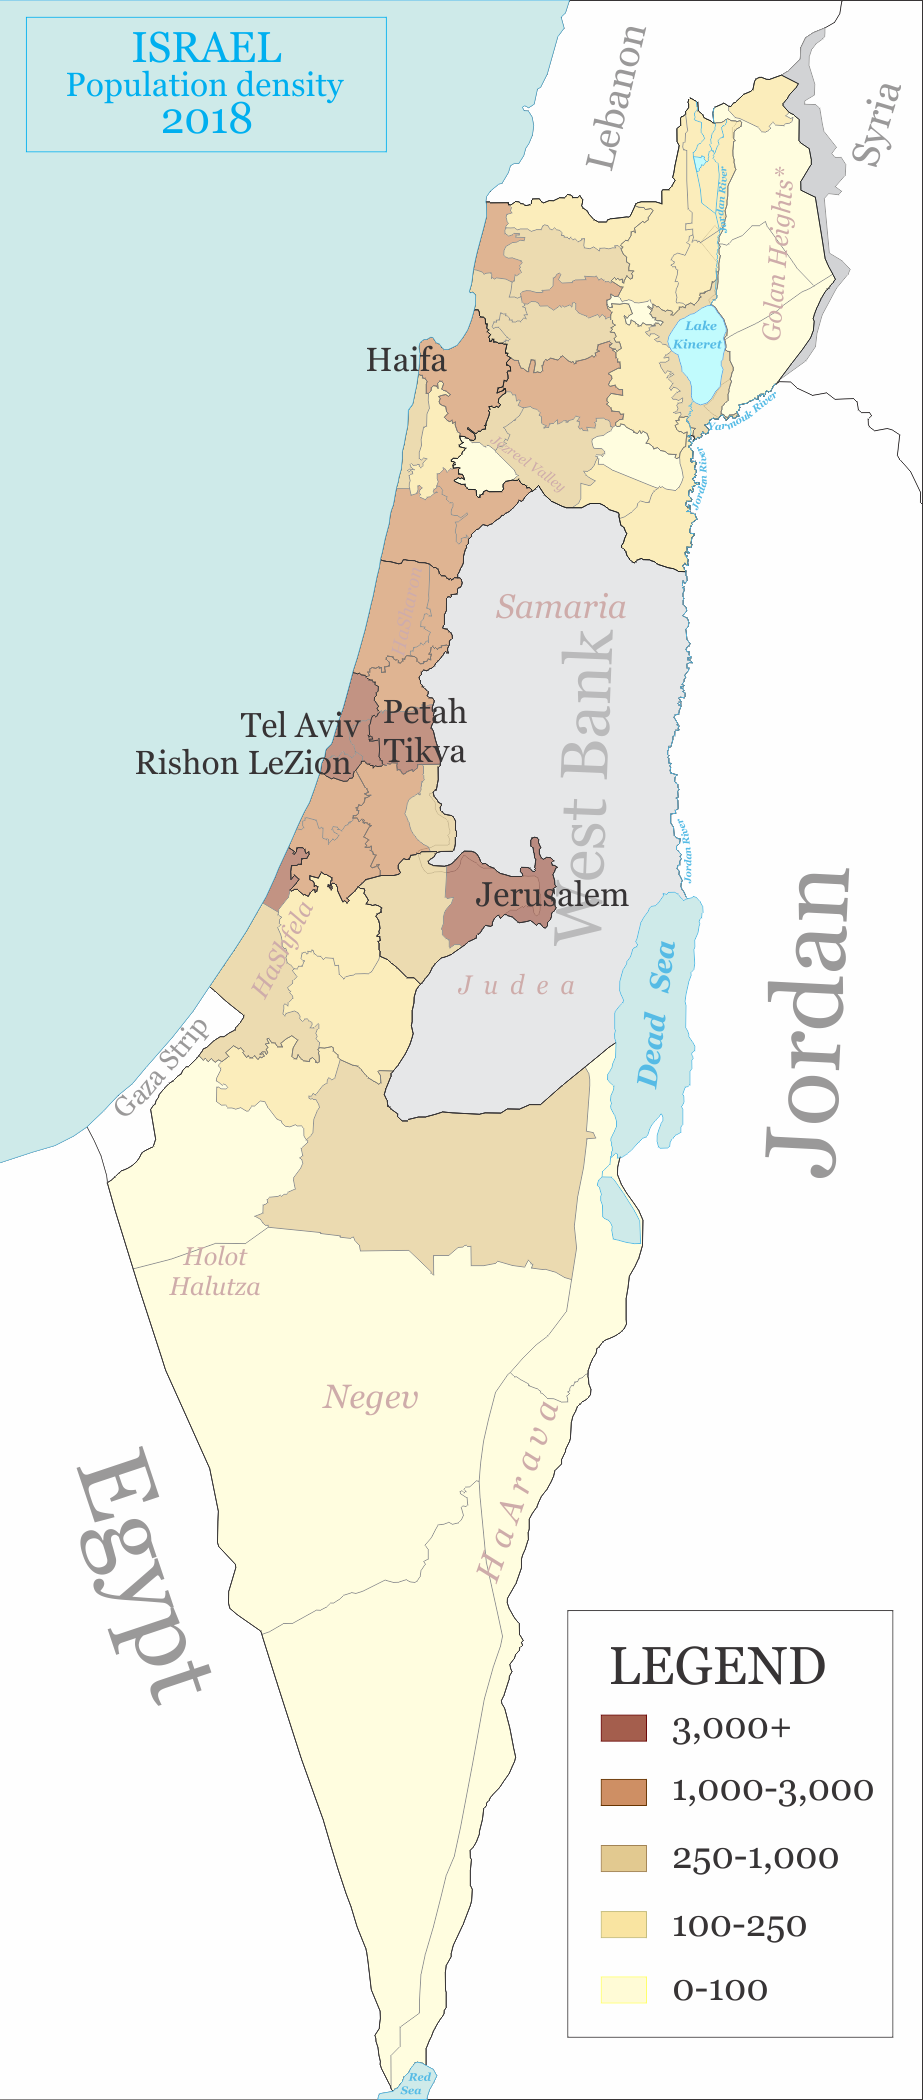
\includegraphics[height=0.42\textheight]{plot/Israel_population_density_2018.png}
    \caption{Population density of Israel (2018, people per km\textsuperscript{2}).
             The coastal plain from Haifa to Ashdod holds most of the
             population; we use the weather at Haifa, Tel~Aviv and
             Jerusalem.}
    \label{fig:pop-density}
\end{figure}

\subsection{The Dataset}

We combine three sources at a common 5-minute resolution, from 1~April~2023
to 31~December~2025; to our knowledge this is the first public dataset of the
Israeli market that aligns them.

\begin{itemize}
    \item \textbf{Demand and the operator's forecast} (Noga, the Israeli
          system operator~\parencite{noga}): national demand every 5~minutes
          and the \emph{real} day-ahead forecast Noga publishes and uses in
          the market---a strong, operational baseline.
    \item \textbf{Day-ahead prices} (Noga~\parencite{noga_smp}): the
          half-hourly unconstrained system marginal price (SMP), the
          market-clearing price $\pi^{\mathrm{DA}}_t$; each 5-minute slot gets
          the price of its settlement period.  (The constrained SMP adds
          redispatch spikes caused by local transmission limits, which a
          national forecast does not affect.)  It averages
          137.5~\textsc{nis}/MWh (\$39.9/MWh) and ranges from 41 to 505.
    \item \textbf{Weather} (Israel Meteorological Service~\parencite{ims}):
          temperature, wet-bulb temperature and relative humidity at Haifa,
          Jerusalem and Tel~Aviv (Figure~\ref{fig:pop-density}).
\end{itemize}

Table~\ref{tab:dataset-stats} summarises the data.  The average load is
9{,}167~MW (about 80~TWh per year).

\paragraph*{The operator's forecast is built for accuracy.}  Noga's forecast
is accurate ($R^2\approx0.98$) and, like a model trained on the squared error,
unbiased and nearly symmetric (Figure~\ref{fig:noga-errors}): the mean error
is $+25$~MW against a standard deviation of 436~MW, and demand exceeds the
forecast in 53\% of the slots.  For accuracy this is ideal; for cost it is
not.  With shortfalls several times more expensive than surpluses, the
cost-optimal forecast is a high quantile (Section~\ref{sec:newsvendor}), and a
forecast centred on the mean falls short about half of the time.

\paragraph*{The uncertainty is not uniform.}  The cost-optimal margin
$F_t^{-1}(\tau_t)-\mathbb{E}[y_t]$ grows with the spread of the demand as
well as with the price.  This spread varies widely: the operator's error
ranges from 1.8\% to 4.8\% MAPE across the hours of the week (standard
deviation 181 to 658~MW, Figure~\ref{fig:error-heatmap}).  It is highest on
the weekend mornings, Friday and Saturday 8:00--15:00, and lowest at night.
A single margin cannot fit both, and a correction per hour of the day (C2,
Section~\ref{sec:compared}) cannot tell a Friday from a Tuesday.  A model
that sees the calendar, the weather and yesterday's price can set its margin
from both the uncertainty and the price.

\begin{figure}[t]
    \centering
    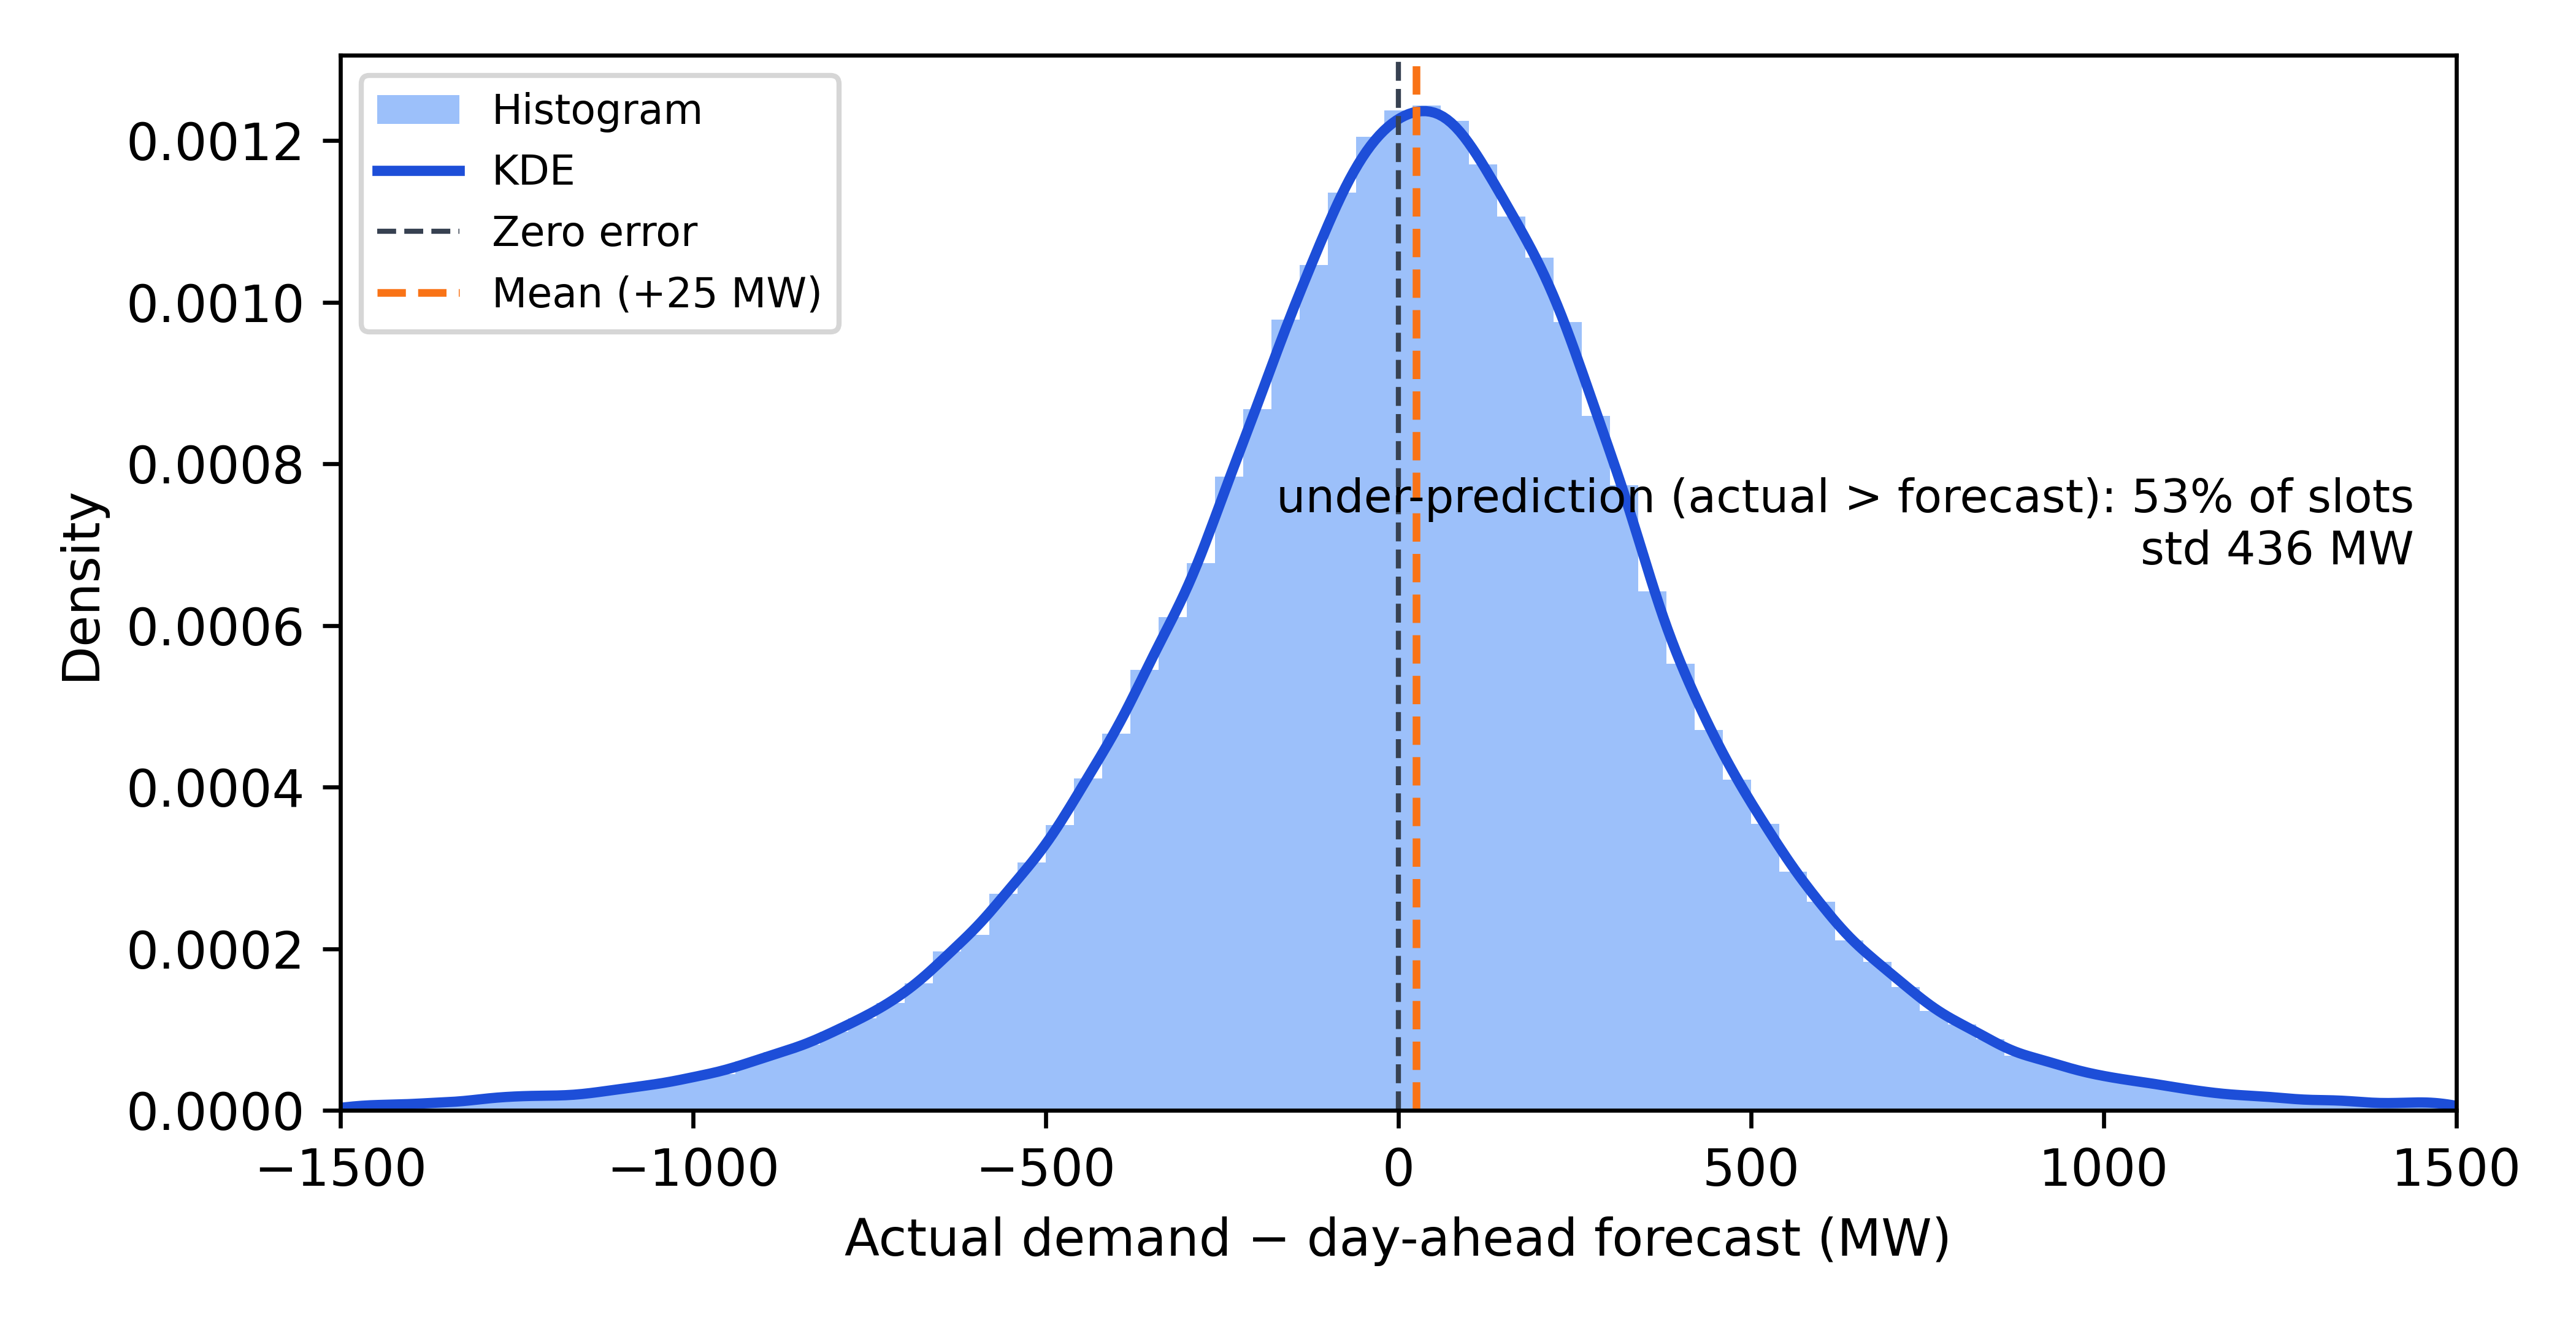
\includegraphics[width=0.85\linewidth]{plot/demand_vs_forecast_kde_histogram.png}
    \caption{Error of the operator's day-ahead forecast (actual minus
             forecast, 5-minute slots, April 2023--December 2025, shown
             within $\pm$1{,}500~MW).  Like a forecast trained on the squared
             error, it is centred near zero and falls short in about half of
             the slots, far from the high quantile that the asymmetric cost
             calls for.}
    \label{fig:noga-errors}
\end{figure}

\begin{figure}[t]
    \centering
    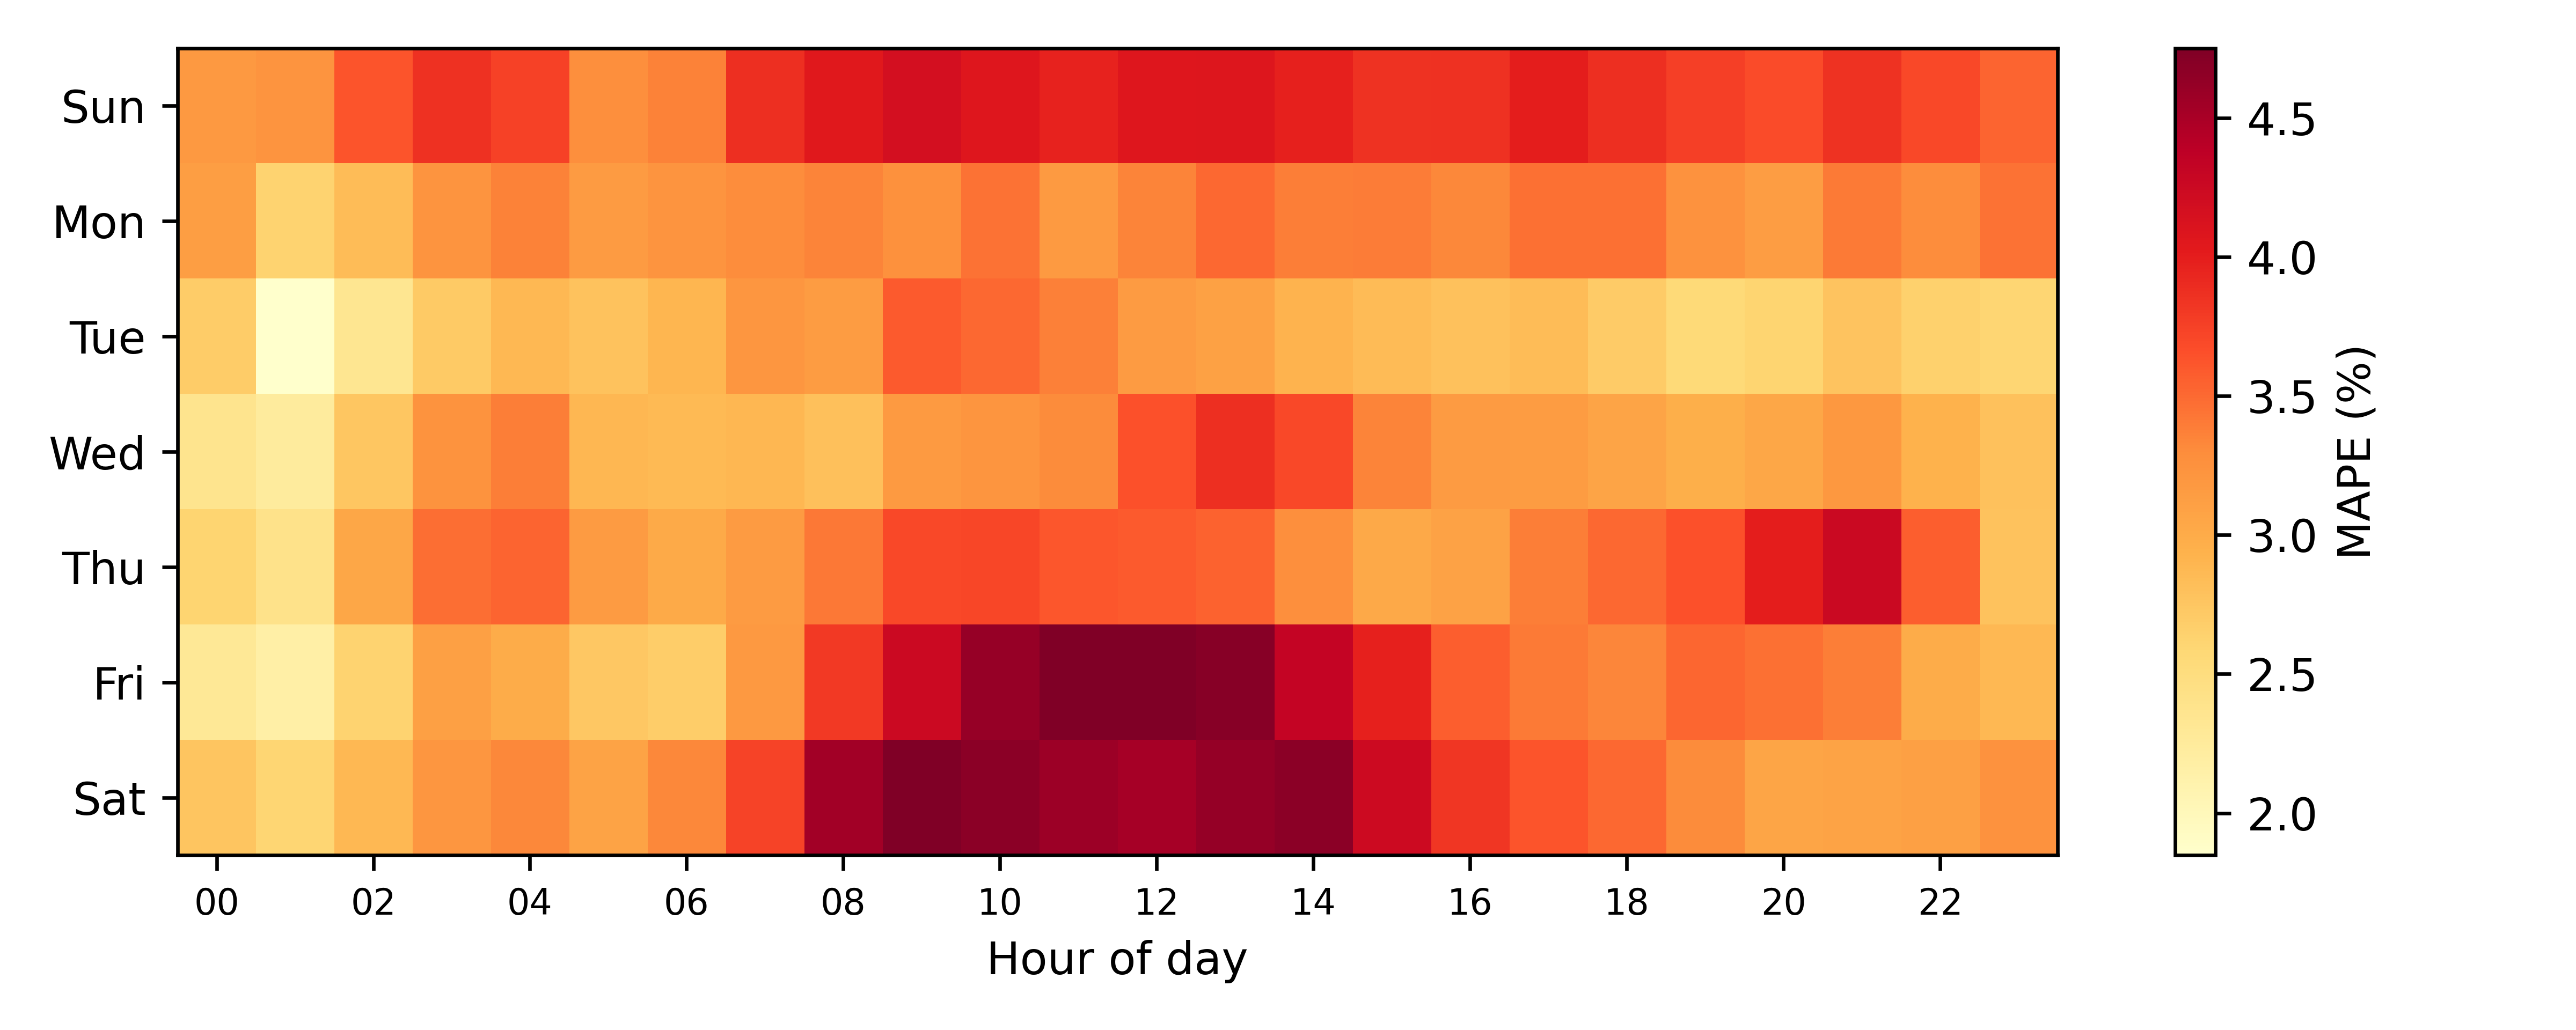
\includegraphics[width=0.9\linewidth]{plot/error_heatmap_percent.png}
    \caption{Mean absolute percentage error of the operator's day-ahead
             forecast by day of week and hour of day.  The uncertainty, and
             with it the cost-optimal margin, varies with the calendar: it is
             highest on the weekend (Friday--Saturday) mornings.}
    \label{fig:error-heatmap}
\end{figure}

\begin{table}[t]
    \centering
    \small
    \caption{Daily summary statistics (1{,}006 days).  $^{*}$Three days with
    an anomalous published forecast (17--19 June 2024) are excluded.}
    \label{tab:dataset-stats}
    \begin{tabular}{lrrrrr}
        \toprule
        \textbf{Variable} & \textbf{Mean} & \textbf{Std} &
        \textbf{Min} & \textbf{Median} & \textbf{Max} \\
        \midrule
        Demand (GWh/day)                       & 219.9 & 37.4 & 147.8 & 211.8 & 342.4 \\
        Operator forecast error (GWh/day)$^{*}$ & $+0.6$ & 6.3 & $-40.1$ & $+0.6$ & $+31.4$ \\
        Day-ahead price (\textsc{nis}/MWh)     & 138 & 26 & 85 & 133 & 245 \\
        Temperature, Tel~Aviv ($^\circ$C)      & 23.2 & 4.8 & 9.6 & 23.7 & 32.1 \\
        \bottomrule
    \end{tabular}
\end{table}

\subsection{Compared Models}
\label{sec:compared}

The data are split chronologically: training on April~2023--December~2024
(\nTrain{} slots) and testing on 2025 (\nTest{} slots).  All learned models
share the network of Figure~\ref{fig:model}, so differences come from how
demand and prices enter training, not from the architecture:

\begin{itemize}
    \item \textbf{MSE}: demand only, trained on the squared error---the
          conventional accuracy-oriented forecaster.
    \item \textbf{Pinball opt}: demand only, trained on the pinball loss at
          the single best constant quantile,
          $\tau^*=\mathbb{E}[c^u]/(\mathbb{E}[c^u]+\mathbb{E}[c^o])=0.864$
          from the training prices---the fixed-asymmetry approach of the
          cost-oriented literature.
    \item \textbf{Joint MSE}: the full network, with the price head, but with
          the demand trained on the squared error---a joint load-and-price
          forecaster trained for accuracy~\parencite{shayeghi2015simultaneous,
          li2024joint}.
    \item \textbf{Unified cost model} (proposed): the full network trained on
          the excess cost and the price loss.
    \item \textbf{Noga}: the operator's published forecast.
\end{itemize}

\paragraph*{Post-hoc corrections.}  To test whether the benefit can be had
more cheaply, we correct the accuracy-trained forecasts to the cost after
training, fitting each correction on the model's own training-set forecasts
at the realised prices: \textbf{C1}, a global affine map $a\hat y+b$;
\textbf{C2}, an affine map per hour of the day, started from the exact
cost-optimal shift of each hour (a cost-weighted quantile of its errors,
Equation~\eqref{eq:weighted_quantile}); and, for Joint MSE, a
\textbf{$\hat\tau$ shift}, which uses the model's own price forecasts: the
training slots are split into deciles of the predicted quantile
$\hat\tau_t$ (Equation~\eqref{eq:optimal_threshold}), and each decile gets its
own cost-optimal shift.  This last baseline is the textbook
\emph{forecast-then-optimise} use of a joint load-and-price forecast.  The
proposed model is never corrected.

\paragraph*{Evaluation.}  The metric is the excess cost
(Equation~\eqref{eq:excess}) on the test year, split into its under- and
over-prediction parts, in million US dollars per year at
3.45~\textsc{nis}/\$ (the 2025 average).  We also report MAE, RMSE and
coverage $P(y_t\le p_t)$.  Each learned model is trained with three seeds
(mean $\pm$ standard deviation), with one draw of the imbalance prices.
Differences in daily cost (averaged over seeds) are tested with the
Diebold--Mariano test~\parencite{diebold1995comparing} with a Newey--West
variance (lag 7 days).


\section{Results}\label{sec:evaluation}
\subsection{Main Results}
\label{sec:main-results}

Table~\ref{tab:main} reports the test-year cost of every model.  The unified
model is the cheapest, at \$49.5$\pm$1.4 million per year, and its advantage
over every alternative is statistically significant.  Each of its three seeds
(\$48.0, 50.7 and 49.9 million) is cheaper than every run of every baseline;
the closest is a Joint MSE~+~C2 run at \$52.2 million.

\begin{table}[t]
    \centering
    \small
    \setlength{\tabcolsep}{4pt}
    \caption{Excess cost on the test year 2025 (million US\$ per year; mean
             $\pm$ standard deviation over three seeds), split into
             under- and over-prediction.  MAE and RMSE in MW; coverage
             $=P(y_t\le p_t)$.  $\Delta$: cost of the unified model minus that
             of the row, with the Diebold--Mariano $p$-value.}
    \label{tab:main}
    \resizebox{\linewidth}{!}{%
    \begin{tabular}{lrrrrrrrr}
        \toprule
        \textbf{Model} & \textbf{Cost} & \textbf{Under} & \textbf{Over} &
        \textbf{MAE} & \textbf{RMSE} & \textbf{Cov.} & $\boldsymbol{\Delta}$ &
        $\boldsymbol{p}$ \\
        \midrule
        \multicolumn{9}{l}{\textit{Operator's forecast}} \\
        Noga                & 76.5 & 61.0 & 15.5 & 294 & 416 & 0.51 & $-27.0$ & $<$0.001 \\
        Noga + C1           & 62.4 & 20.2 & 42.3 & 446 & 544 & 0.86 & $-12.9$ & 0.002 \\
        Noga + C2           & 61.1 & 20.8 & 40.4 & 434 & 536 & 0.86 & $-11.6$ & 0.008 \\
        \midrule
        \multicolumn{9}{l}{\textit{Demand only, trained for accuracy}} \\
        MSE                 & $100.9\pm9.3$ & 90.8 & 10.1 & 265 & 398 & 0.44 & & \\
        MSE + C1            & $59.0\pm2.1$ & 32.3 & 26.7 & 334 & 454 & 0.78 & $-9.5$ & $<$0.001 \\
        MSE + C2            & $56.2\pm2.6$ & 30.3 & 25.9 & 323 & 447 & 0.76 & $-6.7$ & $<$0.001 \\
        \midrule
        \multicolumn{9}{l}{\textit{Demand only, fixed cost asymmetry}} \\
        Pinball opt         & $54.8\pm2.1$ & 21.9 & 32.9 & 379 & 518 & 0.85 & $-5.2$ & $<$0.001 \\
        \midrule
        \multicolumn{9}{l}{\textit{Joint demand and price, trained for accuracy}} \\
        Joint MSE                    & $96.0\pm15.3$ & 86.4 & 9.6 & 259 & 384 & 0.42 & & \\
        Joint MSE + $\hat\tau$ shift & $54.3\pm0.6$ & 29.9 & 24.4 & 307 & 422 & 0.74 & $-4.8$ & $<$0.001 \\
        Joint MSE + C2               & $52.6\pm0.3$ & 27.6 & 25.0 & 310 & 430 & 0.75 & $-3.1$ & 0.004 \\
        \midrule
        \multicolumn{9}{l}{\textit{Joint demand and price, trained on the cost (proposed)}} \\
        \textbf{Unified cost model} & $\mathbf{49.5\pm1.4}$ & 20.1 & 29.4 & 333 & 461 & 0.81 & & \\
        \bottomrule
    \end{tabular}}
\end{table}

\paragraph*{Accuracy is not value.}  The accuracy-trained models are the most
accurate---Joint MSE has the lowest MAE (259~MW), and even plain MSE beats the
operator (265 vs.\ 294~MW)---but, used as they are, the most expensive
(\$96--101 million), because they fall short 56--58\% of the time while a
shortfall costs about six times more than a surplus.  The same holds for the
operator, whose forecast is centred like an accuracy-trained one
(Figure~\ref{fig:noga-errors}): 80\% of its cost comes from shortfalls.

\paragraph*{Post-hoc correction is not enough.}  Correcting the forecasts
after training removes most of the shortfall cost, but the unified model is
still 12\% cheaper than MSE~+~C2 and 19\% cheaper than Noga~+~C2.  A
correction that depends only on the hour cannot tell an expensive afternoon
from a cheap one.

\paragraph*{A fixed asymmetry is not enough.}  Pinball opt knows that
shortfalls are expensive and has the lowest shortfall cost of the learned baselines,
but it buys the same 86\% cover in every slot, pays for it with the highest
surplus cost, and stays 10\% more expensive than the unified model.

\paragraph*{Joint forecasting for accuracy is not enough.}  The strongest
alternative is the joint load-and-price network trained for accuracy and then
corrected, either by its own price forecasts ($\hat\tau$ shift) or per hour
(C2).  With the \emph{same} network, inputs and price head, the unified model
is 6\% cheaper ($p=0.004$).  The only difference is that its demand head is
trained on the price-weighted cost: knowing the price is not enough; the
model must also learn how much cover each price buys, given how uncertain the
demand is in that slot.

\subsection{Why It Works: the Margin Follows the Price}
\label{sec:mechanism}

The cost-optimal margin should grow with the price
(Section~\ref{sec:newsvendor}).  Table~\ref{tab:price-thirds} shows that the
unified model's margin does, from 212~MW in the cheapest third of the slots to
281~MW in the most expensive third.  The fixed-asymmetry model does the
opposite, and the corrected accuracy models barely move.  The unified model is
the cheapest in every third, and it saves the most where it matters most: in
the most expensive third, \$7--15 million per year over the learned baselines
and \$24 million over Noga~+~C2.

\begin{table}[t]
    \centering
    \small
    \caption{Mean safety margin (forecast minus demand, MW) and cost
             (million US\$ per year) by thirds of the test slots sorted by
             day-ahead price (mean over seeds).}
    \label{tab:price-thirds}
    \begin{tabular}{lrrrrrr}
        \toprule
        & \multicolumn{3}{c}{\textbf{Margin (MW)}} &
          \multicolumn{3}{c}{\textbf{Cost (M\$/year)}} \\
        \cmidrule(lr){2-4}\cmidrule(lr){5-7}
        \textbf{Model} & Low & Mid & High & Low & Mid & High \\
        \midrule
        Noga                & $-141$ & $-9$ & 115 & 38.3 & 52.5 & 138.8 \\
        Noga + C2           & 264 & 362 & 421 & 31.4 & 46.1 & 105.9 \\
        MSE + C2            & 181 & 195 & 212 & 28.8 & 42.0 &  97.7 \\
        Pinball opt         & 352 & 296 & 260 & 31.3 & 43.2 &  89.8 \\
        Joint MSE + C2      & 179 & 181 & 208 & 27.0 & 41.2 &  89.6 \\
        \textbf{Unified cost model} & 212 & 241 & 281 & \textbf{25.4} & \textbf{40.8} & \textbf{82.4} \\
        \bottomrule
    \end{tabular}
\end{table}

\paragraph*{Price forecasts.}  Table~\ref{tab:price} compares the unified
model's price forecasts with those of Joint MSE and with a naive forecast,
yesterday's day-ahead price (scaled by the typical training-set ratios for the
surplus and shortfall prices).  On the relative squared error it is trained
on, the unified model beats both on all three prices, and its forecast of the
cost-optimal quantile correlates with the realised one at 0.71, where the
naive forecast carries no information (0.00).  On MAPE, yesterday's price
remains slightly better for the day-ahead price itself (13.5\% vs.\ 14.5\%);
the price head is a single linear layer meant to inform the demand decision,
not to compete with dedicated price models.  A price head that starts from the
naive forecast and learns only a correction lowered the MAPE by about one
point but weakened the quantile forecast (correlation 0.62) and left the cost
unchanged (\$50.0 vs.\ \$49.5 million, $p=0.60$), so we keep the simpler head.

\begin{table}[t]
    \centering
    \small
    \caption{Price forecasts on the test year: MAPE, mean relative squared
             error (RSE, the price head's training loss) and the correlation
             between the predicted and realised cost-optimal quantile
             (mean over three seeds).}
    \label{tab:price}
    \resizebox{\linewidth}{!}{%
    \begin{tabular}{lrrrrrrr}
        \toprule
        & \multicolumn{3}{c}{\textbf{MAPE} (\%)} & \multicolumn{3}{c}{\textbf{RSE}} & \\
        \cmidrule(lr){2-4}\cmidrule(lr){5-7}
        \textbf{Model} & $\pi^{\mathrm{DA}}$ & $\pi^{o}$ & $\pi^{u}$ &
        $\pi^{\mathrm{DA}}$ & $\pi^{o}$ & $\pi^{u}$ &
        \textbf{corr}$(\hat\tau,\tau)$ \\
        \midrule
        Naive (yesterday's price)   & \textbf{13.5} & \textbf{14.1} & 43.0 & 0.044 & 0.046 & 0.281 & 0.00 \\
        Joint MSE                   & 15.6 & 15.8 & 30.7 & 0.040 & 0.041 & 0.149 & 0.70 \\
        \textbf{Unified cost model} & 14.5 & 14.8 & \textbf{29.6} & \textbf{0.036} & \textbf{0.037} & \textbf{0.147} & \textbf{0.71} \\
        \bottomrule
    \end{tabular}}
\end{table}

\subsection{Savings: Israel and a US-Scale Projection}
\label{sec:savings}

Table~\ref{tab:savings} translates the cost differences into annual savings.
Replacing the operator's published forecast with the unified model would save
about \$27 million per year in Israel: \$41 million of avoided shortfall cost,
in exchange for \$14 million of extra surplus.  This is 35\% of the excess
cost, 0.86\% of the \$3.1 billion day-ahead energy bill, \$0.33 per MWh
consumed and \$2.65 per resident.  Even against the operator's forecast after
the best correction (Noga~+~C2) the saving is \$11.6 million per year, now
mainly from buying less unnecessary surplus.

\begin{table}[t]
    \centering
    \small
    \caption{Annual savings of the unified model on the test year (positive:
             the unified model is cheaper), split into under- and
             over-prediction, and normalised per MWh consumed (81~TWh) and per
             resident (10.2~million).  The last column projects the saving per
             MWh to US consumption (about 4{,}100~TWh per year).}
    \label{tab:savings}
    \resizebox{\linewidth}{!}{%
    \begin{tabular}{lrrrrrrr}
        \toprule
        \textbf{Compared with} & \textbf{M\$/year} & \textbf{Under} &
        \textbf{Over} & \textbf{\% of DA bill} & \textbf{\$/MWh} &
        \textbf{\$/resident} & \textbf{US, B\$/year} \\
        \midrule
        Noga (as published) & 27.0 & 40.8 & $-13.9$ & 0.86\% & 0.33 & 2.65 & 1.4 \\
        Noga + C2           & 11.6 &  0.6 &  11.0   & 0.37\% & 0.14 & 1.14 & 0.6 \\
        MSE + C2            &  6.7 & 10.1 &  $-3.5$ & 0.21\% & 0.08 & 0.65 & 0.3 \\
        Pinball opt         &  5.2 &  1.7 &   3.5   & 0.17\% & 0.06 & 0.52 & 0.3 \\
        Joint MSE + C2      &  3.1 &  7.5 &  $-4.4$ & 0.10\% & 0.04 & 0.30 & 0.2 \\
        \bottomrule
    \end{tabular}}
\end{table}

\paragraph*{A US-scale projection.}  Israel is a small market.  The excess
cost scales with the energy traded and with the price level, and the average
US wholesale price, about \$40/MWh in 2025~\parencite{eia_wholesale2025}, is
close to the Israeli \$39.9/MWh.  Scaling the saving per MWh to US consumption
of about 4{,}100~TWh per year~\parencite{eia_steo} gives roughly \$1.4 billion
per year against an uncorrected operator-style forecast and \$0.6 billion
against a corrected one; scaling per resident instead (about 340~million)
gives \$0.9 and \$0.4 billion.  The US market is fragmented into regional
markets with their own designs, so these numbers only illustrate the order
of magnitude: \emph{hundreds of millions to over a billion dollars per year}.

All savings depend on the level of the synthetic imbalance prices
(Section~\ref{sec:synthetic-prices}) and should be read as estimates under
the stated cost model rather than measurements.


\section{Conclusion}\label{sec:conclusion}
\subsection{Summary of Findings}

This paper addressed day-ahead electricity demand forecasting under asymmetric
operational costs using a 3-year national-scale, high-resolution dataset of
electricity use prediction and actual consumption.  Our main findings are:

\begin{enumerate}
    \item \textbf{Asymmetric costs are pervasive and substantial.}  In
          electricity markets, the costs of under-predicting demand substantially
          exceed those of over-prediction.  Empirically plausible cost ratios
          $c_u/c_o\in[5,20]$ have a large impact on the optimal forecasting
          strategy.

    \item \textbf{The newsvendor framework provides a principled optimality
          condition.}  The cost-minimising procurement level corresponds to a
          specific quantile $\tau^*=c_u/(c_u+c_o)$ of the conditional demand
          distribution.  For a cost ratio of~5, this yields $\tau^*\approx 0.833$,
          i.e.\ the 83.3rd percentile of demand --- a systematic upward shift
          that is normatively \emph{desirable} under asymmetric costs.

    \item \textbf{Asymmetric loss training effectively targets the cost-minimising
          quantile.}  A feedforward neural network trained with a cost-sensitive asymmetric loss
          function (specifically, a non-linear variant of the pinball loss) at
          the appropriate quantile achieves lower expected operational cost than
          an L1-trained neural network baseline.  The cost
          reduction is consistent across a wide range of synthetic cost function
          parameters.

    \item \textbf{Symmetric loss is a misleading evaluation metric under asymmetric costs.}
          The L1-trained neural network achieves lower MAE than the asymmetric-loss model
          yet incurs higher expected operational cost.  Practitioners should adopt
          cost-sensitive metrics such as asymmetric loss or expected operational
          cost for model selection and evaluation.

    \item \textbf{Post-hoc calibration helps but does not substitute for
          cost-aware training.}  A global affine correction fitted to the
          operational cost recovers much of the gap on asymmetric metrics, but
          cannot match a model trained end-to-end, because it cannot adapt the
          upward bias to the input-conditional structure of forecast error.

    \item \textbf{The approach is practical and improves on the operational
          forecast.}  Our model is a small, open-source feedforward network that
          trains in minutes on commodity hardware.  Even though predictive
          accuracy was not an objective of this work, it improves on the Noga
          operational forecast not only on cost-sensitive metrics but also under
          symmetric error metrics such as MSE; we believe substantial
          further gains in this aspect are readily achievable.  Together with a demonstrated
          economic benefit, this makes the method realistic to adopt in practice.
\end{enumerate}

\subsection{Implications for Market Participants and Policymakers}

\textbf{For market participants} (electricity retailers, large consumers,
aggregators), the key takeaway is that standard forecasting tools optimised for
MSE are likely to systematically under-procure electricity, exposing them to
avoidable real-time market risk.  Incorporating asymmetric cost modelling ---
through direct asymmetric-loss training or post-hoc quantile adjustment --- can
yield meaningful reductions in procurement costs with negligible additional
computational overhead.

\textbf{For grid operators} (transmission system operators, independent system
operators), the implication is that incentivising cost-sensitive forecasting
among market participants could improve overall system reliability.  If all
participants systematically under-forecast demand, the system operator faces
persistent shortfalls in committed reserves.  Regulatory frameworks that reward
forecast accuracy measured by cost-sensitive metrics, rather than MSE, would
align private incentives with system reliability objectives.

\textbf{For policymakers}, our results support the inclusion of cost-sensitive
forecasting requirements in market design rules.  For example, mandatory reporting of asymmetric (pinball) loss at relevant
quantiles, alongside MSE, would provide a richer picture of forecast quality
that better reflects operational costs.

\subsection{Limitations}

Along with these positive findings, this work also has several limitations, as follows:

\begin{itemize}
    \item \textbf{Synthetic imbalance prices.}  The day-ahead prices are real,
          but Noga does not publish real-time imbalance prices for the study
          period, so the under- and over-prediction prices are generated
          synthetically.  Although the generator is anchored on the real
          day-ahead price and our conclusions are robust to its parameters
          (Section~\ref{sec:sensitivity}), the absolute savings depend on the
          assumed imbalance-price level and should be read as an estimate under
          the stated cost model.

    \item \textbf{Known day-ahead price.}  We treat the SMP as the
          market-clearing price and assume that it, and the over-prediction
          price, are known when the procurement quantity is chosen.  In the
          Israeli market the SMP is itself derived from the operator's
          day-ahead schedule; a participant who must forecast the price would
          face additional uncertainty.

    \item \textbf{Price-taker assumption.}  We evaluate the cost of a single
          procurement decision at given prices and ignore the feedback of a
          changed forecast on the prices themselves.  For the system operator,
          whose forecast drives the schedule, this feedback is not negligible.

    \item \textbf{Point forecasts only.}  Our neural network produces a single scalar
          forecast at the (price-dependent) target quantile.  A richer approach
          would estimate the full predictive distribution, enabling uncertainty
          quantification.
\end{itemize}

\subsection{Directions for Future Research}

\begin{enumerate}
    \item \textbf{Distributional forecasting.}  Training models to output full
          predictive distributions (via normalising flows, conformal prediction,
          or Bayesian deep learning) would enable the optimal quantile to be
          selected adaptively as a function of current cost parameters.  We regard
          this, rather than training against a fixed cost function, as the proper
          long-term formulation of the problem, for the reasons set out in the
          concluding remarks below.

    \item \textbf{Nonlinear and non-smooth cost functions.}  Step-function or
          tiered cost structures require optimisation approaches beyond the
          pinball loss, such as distributionally robust optimisation or stochastic
          programming.

    \item \textbf{Online and adaptive learning.}  Adaptive algorithms that update
          the forecasting model in real time as market conditions change would be
          valuable for practical deployment.

    \item \textbf{Richer temporal modelling.}
          Our model already operates at fine (5-minute) granularity but treats
          each target slot largely independently.  Explicitly modelling
          intra-day and cross-day demand dynamics, for example with Transformer
          architectures~\parencite{vaswani2017attention} or temporal
          convolutional networks, could better exploit the structured
          hour-of-week error pattern documented in
          Section~\ref{sec:forecast-error-dist}.

    \item \textbf{Joint price and demand forecasting.}  Relaxing the
          known-price assumption by forecasting the day-ahead price jointly with
          demand, and modelling the dependence of imbalance prices on the
          system-wide forecast error (scarcity pricing), are natural next
          steps.

    \item \textbf{Multi-product forecasting.}  In practice, electricity retailers
          must manage procurement across multiple products (day-ahead energy,
          reserves, ancillary services) with correlated costs and demands.  A
          joint cost-sensitive forecasting framework would be a substantial
          extension.

    \item \textbf{Real imbalance prices.}  Collaboration with market
          participants or the operator to obtain actual imbalance settlement
          prices would remove the need for synthetic under- and
          over-prediction prices.
\end{enumerate}

\subsection{Concluding Remarks}

Electricity demand forecasting sits at the intersection of time series analysis,
optimisation under uncertainty, and energy economics.  As markets become more
complex, driven by variable renewable energy, demand response, and distributed
storage, the costs of forecast errors are likely to increase, making
cost-sensitive forecasting ever more important.

This work demonstrates that a conceptually simple modification --- giving the
forecaster the market prices it will be settled at, and training it on the
resulting procurement cost instead of MSE --- leads to meaningful improvements in
operational cost without sacrificing computational tractability.  Because the
prices enter as inputs, a single model serves the whole range of cost
asymmetries that the market produces, rather than one fixed ratio chosen in
advance.

A complementary formulation is to \emph{decouple estimation from
decision-making}: first predict the full \emph{conditional distribution} of
demand, and then optimise the procurement quantity at decision time against the
prevailing prices.  Our price-aware newsvendor baseline (C2) is a simple
instance of this idea; our results suggest that, with the data available, the
unified model exploits the interaction between prices and the other features
better than such a two-stage approach.  Combining the two --- distributional
models that are themselves trained on price-weighted objectives --- is a
promising direction for future work.
We hope these findings contribute to a broader shift
towards cost-aware forecasting practices in the electricity industry and stimulate
further research at the intersection of machine learning and energy systems
optimisation.


% Elsevier's standard statement; it goes at the end of the manuscript,
% before the references.
\section*{Declaration of generative AI and AI-assisted technologies in the
manuscript preparation process}
During the preparation of this work the authors used Claude (Anthropic) in
order to improve the language and readability of the manuscript.  The
research itself---the problem formulation, the model, the experiments and
the analysis---was conceived and carried out by the authors.  After using
this tool, the authors reviewed and edited the content as needed and take
full responsibility for the content of the published article.


\FloatBarrier
\printbibliography

\end{document}
